\documentclass[]{article}
\usepackage{tikz}
\usepackage{geometry}[margins = 0.5 in]
\usepackage{graphicx}
\usepackage[hyphens,spaces,obeyspaces]{url}
\usetikzlibrary{arrows}
\usepackage{float}
\usepackage{afterpage}
\usepackage{lipsum}
\usepackage{caption}
\usepackage{listings}
\usepackage{listing}
\usetikzlibrary{arrows.meta}
\graphicspath{ {c:/user/lolzk/SParameterGraph1D} }
\graphicspath{ {c:/user/lolzk/Smith Plot for Reflection} }
\graphicspath{ {c:/user/lolzk/Electric Field Normal Graph Image2} }
\graphicspath{ {c:/user/lolzk/Electric Field Normal Graph Image} }
\graphicspath{ {c:/user/lolzk/Quasistatic Magnetic Field Vector Direction Graph Images} }
\graphicspath{ {c:/user/lolzk/OneD Electric Field Normal Graph Image} }
\graphicspath{ {c:/user/lolzk/Unit Cell } }
\title{Using Quasi-static Magnetic Fields and Meta-material Amplifiers to allow for Ubiquitous Wireless Charging}
\author{Jordan Hill \\ David Stover}
\begin{document}
\maketitle
\pagebreak

\begin{abstract}
Quasi-static Magnetic fields are Electromagnetic fields that are created from Quasi-static cavity resonance. Meta-materials are materials that have the ability to allow for high amounts of electric resonance, have the possibility to allow for highly efficient wireless charging, and solve the problem of current wireless charging. This causes the user to be restricted there device always while the device is charging, and not allowing the user the use of mobility while using wireless charging with modern methods. Hypothetically, to make the process of wireless charging hundreds of time more efficient through use of Quasi-static magnetic fields and reflective meta-materials as a use to solve this problem. Simulations for this was done using COMSOL 5.2a, and within that software is where the main work was done for calculating absorption of the Quasi-static magnetic field, along with the permittivity of the meta-material, $\epsilon_s$, and the permeability of the meta-material as well, defined as $\mu_0$. The Implemented experiment results that I obtained from COMSOL, in some cases fit the results I expected from the simulations and in some aspects did not fit the results I expected. The Importance of this project is mainly of how the application of such a method could be extremely useful in making the experience in wireless charging more free and open to the user, and not have the user forced to always keep the device on a pad when charging there device wireless, with current methods of wireless charging today being used.
\end{abstract}

\pagebreak

Wireless Charging, the Pinnacle of refueling devices, free of constraints, nothing holding the user back from being forced to charge with the length of cord limiting there freedom to move around while charging there device. But, a problem is present with Modern Wireless Charging in the current form that it is used in currently, and that is the need for a connection constantly to charge your device. The current method of wireless charging used today is known as Qi Charging. Qi Charging works with the wireless charging device having a built in copper coil. The Copper Coil is attached to the battery of the device, so current is put into the battery correctly while the device is charging. Power is transferred to the device through a Wireless Charging Pad, containing a Copper Coil inside the Pad. Transfer of Power is done between these two coils, using the coil inside the device as an inducting coil, and an alternating electromagnetic field is created. This field is the process responsible for allowing the wireless charging to occur in Qi Charging, and charge the device (Mearin, 2018). But, there is a problem with this process, and that is the lack of mobility, as when you place the device on the pad, you cannot under any circumstances remove it, as if you remove it from the pad, you lose the electromagnetic field that was made between the two coils, one in the pad and the device itself, which stops the charging process itself, which shows the Problem of Mobility with this method of wireless charging comes into play. Now, the answer to this problem is quite simple, and that is with the use of a Material, a special material, and the types of that being referred to as Meta-materials. Meta-materials are special materials, designed to have properties not found in any other modern material that would be found in Nature, and have a variety of properties when produced. Some of these materials have been known to have the ability to reflect electromagnetic waves, and reflect them completely, having no interaction with the Material itself what so ever (Institute of Physics, n.d.). This application of such Meta-materials has great application to solve the problem of mobility with wireless charging. Meta-materials can contain these properties, mainly due to the construction of there unit cells, which make up the fundamental structure of the material itself, and its properties, such as impedance, admittance, and reflective properties of the material. Impedance is the effect of electrical resistance on an electrical component when compared to the alternating current (Wikepedia, 2018), if one is present. The Reflective properties of the material mainly if the material doesn't absorb any of the Electromagnetic waves from the Quasi-static Magnetic field, but reflects them instead rather than absorbing the Electromagnetic waves from the Quasi-static magnetic field. A Meta-material itself, when they are made have something called a unit cell. A unit cell is what the meta-material makes up the design of the cells of the sheet of a meta material, with each space containing the unit cell itself, which is then typically inserted onto a slab of a material, with the unit cells of the Meta-material are placed on. Then, there is a concept known as Quasi-static Cavity Resonance. Quasi-static Cavity Resonance is a method that can be used to create near standing waves for a magnetic field inside a resonant structure, and resonant coupling to smaller receivers that can pick up the charge and are near the structure itself (Chabalko, M. J., Shahmohammadi, M., Sample, 2017).
\linebreak
My project mainly focuses on one thing, and that is making the process of wireless charging more efficient, and more applicable to be used as a main charging method for charging devices rather than a cord method. I did this by attempted to find a way using the concept of Quasi-static cavity resonance, and Quasi-static magnetic fields, to generate a magnetic field that can then be deflected by a set of meta-material reflectors. These Meta-material reflectors would then reflect any waves from the Quasi-static magnetic field, which would then be picked up by the receiver in a device in this case. Once the reflected wave off the meta-material reflector would be picked up by the receiver in the device, the device would charge due to this. The results I would be obtaining from the COMSOL Simulations would allow me to see the total absorption of the waves from the Quasi-static magnetic field that the meta-material had, and also the reflectance that the meta-material unit cell had, which in this case would be graphed in the form of a smith plot, which will be how that is graphed. In summary, my main goal with this project is to find a possibly more efficient method of wireless charging by using Quasi-static magnetic fields and meta-materials, to allow for wireless charging that truly allows for wireless charging on the mobile level that it was always meant to be at. The Main Hypothesis I have about my results are that they will show the method of using meta-materials as a method to allow for wireless charging at a level where you don't have to worry about it always being connected to a pad, and with the use of Quasi-static magnetic fields will be a very efficient process to allow wireless charging at truly mobile distances like it should be.

\section*{Methods and Materials} 
Materials used in this project were quite minimal, due to the centralized nature of it heavily around simulations of the project, before any theoretical modeling was actually done. The start of the project involved me doing mathematical modeling for the theoretical part of this project, which saw me define the main elements of the project, such as the strength of the Quasi-static magnetic field, meta-material related parameters, and other components as well. All of the experimental work was done within the FEM Analysis software, COMSOL 5.2a, with the results from the simulation runs for certain components of the project being exported out for data collection. For finding the T-Test values, or any other statistical values of that matter, the use of python was employed with the help of the python module, \textit{PANDAS}, which is a python module that is used for the purpose of data science and statistics mainly.

\subsection*{Mathematical Modeling}
Mathematical Modeling used within this project worked with many equations, but one of the main ones being for the modeling of the Quasi-static field coming from the main Quasi-static magnetic field generator itself. To define this Generator of the Quasi-static magnetic field, a Cylinder was designed for the theoretical model, which is for the cylinder, the length being symbolized by it being approximately equal to $\Delta$l, as shown here: $\Delta$l $\approx$ 2.4384 m. Visualizing this, a point of displacement for the field was defined to calculate the possible strength, with that point being defined as:
\begin{equation}
\rho =  \left(\begin{array}{c}
x \\
y \\
z 
\end{array}\right)
\end{equation}
with $\rho$ being the point of displacement being used for calculating the strength of the Quasi-static magnetic field at this point of displacement for calculating the strength of it. Along with this, when defined, a current direction is placed going up through the cylinder itself, being defined as $\vec{I}$, and this is repeated twice over the cylinder, the main generator that is, and an equation for this current and the current direction can be defined as:
\begin{equation}
C = \vec{2I} + \vec{I}
\end{equation}
where \textbf{\textit{C}} in this equations is the sum of the vector directions for the current direction of $\vec{I}$. In the equation with $\vec{2I}$, that is defined as both of the current directions summed together, with the $\vec{I}$ being the individual current direction of $\vec{I}$ in the equation. The Purpose of the Equation here is mainly to define the total amount of current, being defined in mA, that being milliamperes, for the given equation, with the adding of the two being used to calculate the current going either in a negative direction into a negative quadrant of the 3D Coordinate plane, or the opposite, with the current going in a positive direction into a positive quadrant. Then, for calculating the point of displacement, and the strength of the Quasi-static Magnetic, use of Biots Savarts law, which is written as:
\begin{equation}
B = \frac{\mu_0I}{4\pi}
\end{equation}
and then for use for the approximation with using the point of displacement to calculate the strength of the Quasi-static Magnetic Field, that can be defined as the following equation, which is: 
\begin{equation}
\rho = x^2+y^2+z^2
\end{equation}
with that to be used in the approximation, for calculating the point of displacement, and with that, we can define an equation for the point of displacement, and in turn the Quasi-static Magnetic field at the point we selected in this case, with this equation being defined as,
\begin{equation}
B = \frac{\mu_0I}{4\pi} \cdot \frac{ \left(\begin{array}{c} 
0 \\
-\Delta\l \\
0 
\end{array}\right) \cdot \left(\begin{array}{c}
x + \frac{\Delta\l}{2} \\
\Delta{y}\ \\
z
\end{array}\right)}{((x + \frac{\Delta\l}{2}) ^ 2 + y^2 + z^2)^\frac{3}{2}} + \frac{\mu_0I}{4\pi}
\linebreak
\cdot \frac{\left(\begin{array}{c}
\Delta\l \\
0 \\
0
\end{array}\right) \cdot \left(\begin{array}{c}
\Delta{x}\ \\
y - \frac{\Delta\l}{2} \\
z
\end{array}\right)}{(x^2 + (y - \frac{\Delta\l}{2})^2 + z^2)^ \frac{3}{2}} + \]
\[\frac{\mu_0I}{4\pi} 
\cdot \frac{\left(\begin{array}{c}
0 \\
\Delta\l \\
0
\end{array}\right) \cdot \left(\begin{array}{c}
x - \frac{\Delta\l}{2} \\
-\Delta{y}\ \\
z
\end{array}\right)}{((x - \frac{\Delta\l}{2})^2 + (-\Delta{y})^2 + z^2)^\frac{3}{2}} + \frac{\mu_0I}{4\pi} \cdot \frac{\left(\begin{array}{c}
-\Delta\l \\
0 \\
0
\end{array}\right) \cdot \left(\begin{array}{c}
-\Delta{x} \\ 
y + \frac{\Delta\l}{2} \\
z^2
\end{array}\right)}{((-\Delta{x})^2 + (y - \frac{\Delta\l}{2})^2 + z^2)^\frac{3}{2}} + \frac{\mu_0I}{4\pi}
\end{equation}
Now, with the equation written above, it can be used to calculate the strength of the magnetic field at the displacement point selected, which is the point $\rho$, and using that point and the equation above, now that we have this equation for that point, and the calculations for the point and the distance to it, which were all calculated here in this case to be constant. Next we have the use of discrete capacitors, which are within the center of the cylinder, below is an example of this, all of the discrete capacitors in the center for the mathematical model is down below: 
\begin{figure}
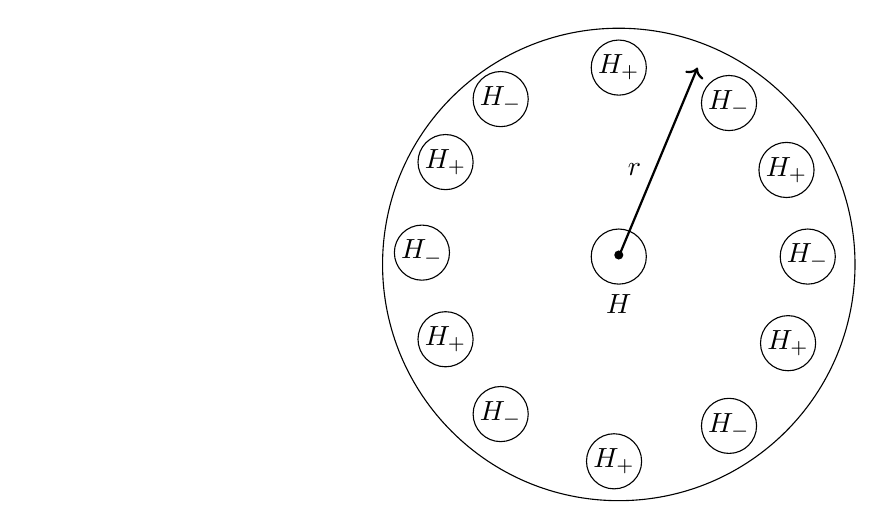
\begin{tikzpicture}
\draw (0.5,3) ellipse (0cm and 0cm);
\draw(8,0) circle(3 cm);
\draw(8,0.1) circle(0.35cm);
\draw[fill](8, 0.12) circle(0.05cm);
\draw(8.2, 1.2) circle(0.00cm) node{$r$};
\draw(8, -0.5) circle(0.00cm) node{$H$};
\draw(5.5,0.15) circle(0.35 cm) node{$H_-$};
\draw(5.8,1.3) circle(0.35 cm) node{$H_+$};
\draw(5.8,-0.95) circle(0.35 cm) node{$H_+$};
\draw(6.5, -1.9) circle(0.35 cm) node{$H_-$};
\draw(6.5, 2.1) circle(0.35 cm) node{$H_-$};
\draw(9.4, 2.05) circle(0.35 cm) node {$H_-$};
\draw(8, 2.5) circle(0.35 cm) node{$H_+$};
\draw(7.94, -2.5) circle(0.35 cm) node{$H_+$};
\draw(9.4, -2.05) circle(0.35 cm) node{$H_-$};
\draw(10.15, -1) circle(0.35 cm) node{$H_+$};
\draw[->, thick, black](8,0.1) -- (9,2.5);
\draw(10.13, 1.2) circle(0.35 cm) node{$H_+$};
\draw(10.4, 0.1) circle(0.35 cm) node{$H_-$};
\end{tikzpicture}
\end{figure}
Here, with the diagram of the discrete capacitors, there is one thing that is not known, and that is the dielectrics of each discrete capacitor. For this, an equation can be used, with finding the dielectrics for each capacitor, and then the capacitance of each capacitor. For this, we can start with the following equation that uses Coulombs constant,
\begin{equation}
V = \frac{\lambda}{4\pi\epsilon_o} \int_{in}^{out} \frac{\vec{H}\cdot \vec{\mu}}{r^2} \cdot dt
\end{equation}
with $V$ being the dielectrics of the discrete capacitors, what it is defined as mainly. Then with the current going out, defined as \textit{out}, being integrated over the current going in, being defined as \textit{in}, and that current direction going through the discrete capacitors, being defined as $\vec{H}$, the current direction and current, is defined as $\vec{\mu}$, with $r^2$ being the $\vec{r}$ coming from the center discrete capacitor that is neither positive or negatively charged. Now with this equation, we can find with the equation being used from above 
\begin{equation}
V =\frac{\lambda}{4\pi\epsilon_o}\int_{in}^{out} \frac{\vec{H}\cdot \vec{\mu}}{r^2} \cdot dt
\end{equation}
and then find with making the $\vec{H}$ into an integral for the + and - charge of each of the capacitors in the diagram shown of the discrete capacitors in the generator, the equation then becomes,
\begin{equation}
V = \int_{H_-}^{H_+} \frac{\lambda}{4\pi\epsilon_o}\int_{in}^{out}\frac{\vec{H} \cdot \vec{\mu}}{r^2} \cdot dt
\end{equation}
with this new equation, use $dt$ as the derivative we integrate the integral $\int_{H_-}^{H_+}$ using this derivative, the equation then becomes,
\begin{equation}
V = \frac{-\lambda}{4\pi\epsilon_o} \int_{in}^{out}\frac{\vec{H} \cdot \vec{\mu}}{r^2} \cdot \biggr|_{H_{-}}^{H_{+}}
\end{equation}
with the differential $dt$ removed, and used to integrate the integral $\int_{H_-}^{H_+}$, it can the equation can then become,
\begin{equation}
V = \frac{\lambda}{4\pi\epsilon_o}\int_{in}^{out} \frac{\vec{H}(+)(-) \cdot \vec{\mu}}{r^2}
\end{equation}
Now, with this new equation found, we can then turn the integral $\int_{in}^{out}$ into a natural logarithm, which when symbolized is $ln$, which then gives us the equation
\begin{equation}
V = \frac{\lambda}{4\pi\epsilon_o} \cdot \ln(\frac{out}{in})\frac{\vec{H}(+)(-) \cdot \vec{\mu}}{r^2}
\end{equation}
due to the presence of the new natural logarithm, $ln$, replacing the integral from the equation before where there was still the integral $\int_{int}^{out}$, which is now the natural logarithm $ln(\frac{out}{in})$. Then, to remove $r^2$ from the equation, we derive it out and have the new equation of, 
\begin{equation}
V = \frac{\lambda}{4\pi\epsilon_o} \ln(\frac{out}{in})\vec{H}(+)(-)\cdot \vec{\mu}
\end{equation}
With the equation for the dielectrics of the capacitors now found, to find the total possible capacitance of each capacitor, the law of capacitance can be used to do this, with the equation for that law being,
\begin{equation}
C = \frac{Q}{V} 
\end{equation}
where $C$ is the total capacitance, which is divided by V, the dielectric of the capacitor in this case, using the capacitance law, we can substitute $Q$ for $\lambda$ in the equation  where $r^2$ is removed, which gives us the equation of,
\begin{equation}
V = \frac{Q}{4\pi\epsilon_o\mu}\ln(\frac{out}{in})\vec{H}(+)(-)
\end{equation}
where $\vec{\mu}$ is carried over and added to the Coulombs constant for the equation, which makes it $V = \frac{Q}{4\pi\epsilon_o\mu}$ due to that. Then, using the law of capacitance, which is $C = \frac{Q}{V}$, and substitute the results we have for $V$, we get the equation of,
\begin{equation}
C = \frac{Q}{\frac{Q}{4\pi\epsilon_o\mu}}\ln(\frac{out}{in})\vec{H}(+)(-)
\end{equation}
with this equation, when we remove $Q$ from the equation and divide it out from the nested fraction of the equation, we get the final equation of,
\begin{equation}
C = \frac{4\pi\epsilon_o\mu}{\ln(\frac{out}{in})}\vec{H}(+)(-)
\end{equation}
we then have the final equation for the total capacitance of each discrete capacitor within the diagram shown earlier in this section. With the total capacitance found for each of the discrete capacitors, we can then go onto finding the total possible energy stored in each discrete capacitor. For this, we can start out by defining the differential, $dQ$, which can be defined as $dQ$ = capacitance of a given capacitor for this function. With this differential, we can define this by placing one of the capacitor onto a 3d coordinate plane, as shown here within the diagram,
\linebreak
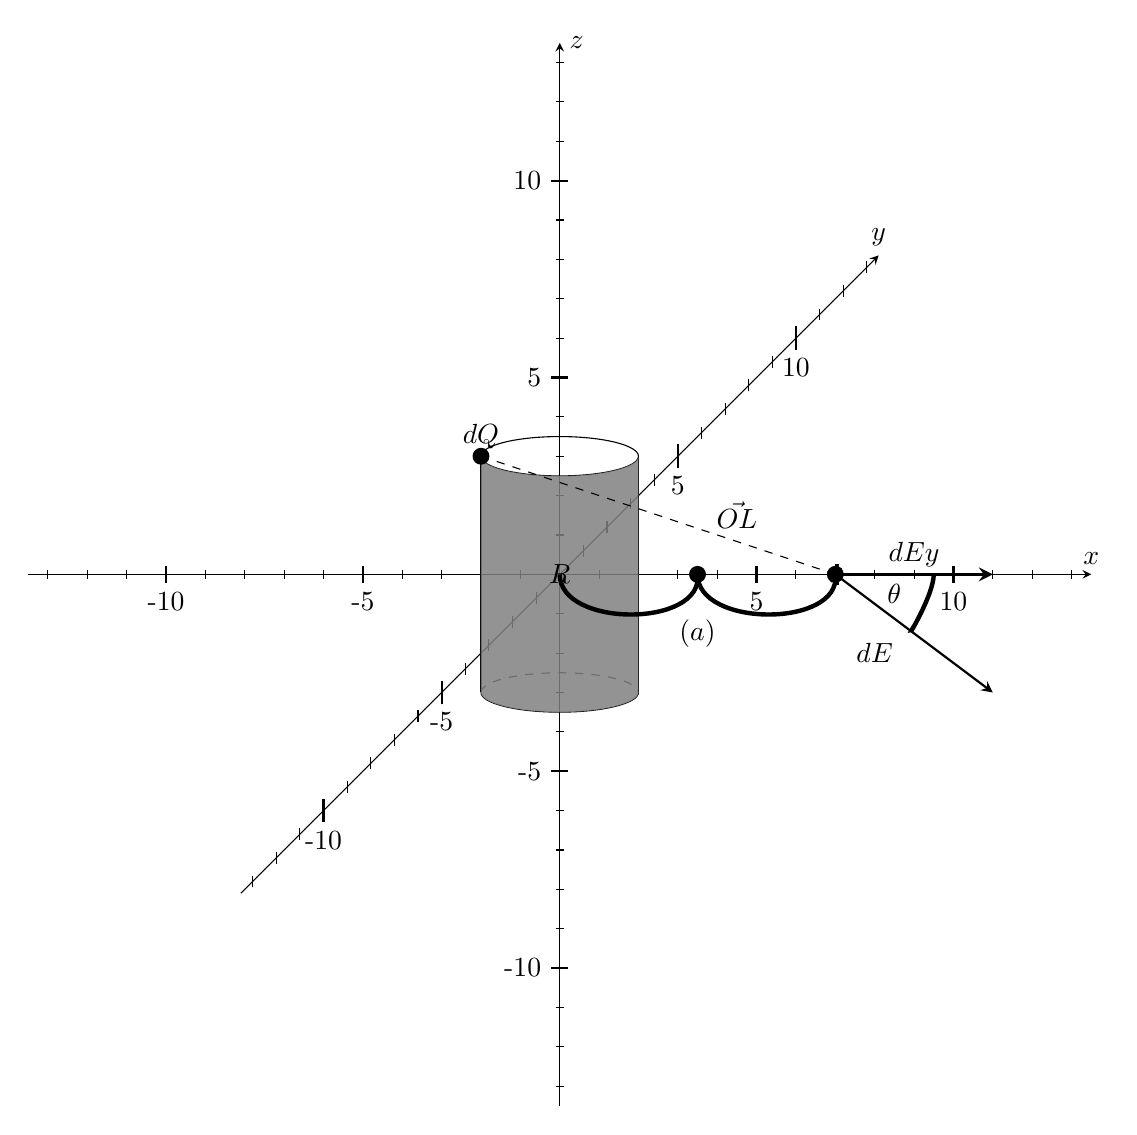
\begin{tikzpicture}[x=0.5cm,y=0.5cm,z=0.3cm,>=stealth]
\draw[->] (xyz cs:x=-13.5) -- (xyz cs:x=13.5) node[above] {$x$};
\draw[->] (xyz cs:y=-13.5) -- (xyz cs:y=13.5) node[right] {$z$};
\draw[->] (xyz cs:z=-13.5) -- (xyz cs:z=13.5) node[above] {$y$};
\foreach \coo in {-13,-12,...,13}
{
	\draw (\coo,-1.5pt) -- (\coo,1.5pt);
	\draw (-1.5pt,\coo) -- (1.5pt,\coo);
	\draw (xyz cs:y=-0.15pt,z=\coo) -- (xyz cs:y=0.15pt,z=\coo);
}
\foreach \coo in {-10,-5,5,10}
{
	\draw[thick] (\coo,-3pt) -- (\coo,3pt) node[below=6pt] {\coo};
	\draw[thick] (-3pt,\coo) -- (3pt,\coo) node[left=6pt] {\coo};
	\draw[thick] (xyz cs:y=-0.3pt,z=\coo) -- (xyz cs:y=0.3pt,z=\coo) node[below=8pt] {\coo};
}
\draw (0,3) ellipse (2 and 0.5);
\draw (-2,3) -- (-2,-3);
\draw (-2,-3) arc (180:360:2 and 0.5);
\draw [dashed] (-2,-3) arc (180:360:2 and -0.5);
\draw (2,-3) -- (2,3);  
\fill [gray,opacity = 0.85] (-2,3) -- (-2,-3) arc (180:360:2 and 0.5) -- (2,3) arc (0:180:2 and -0.5);
\draw (0,0) circle(0 cm) node{$R$};
\draw[fill](7,0) circle(0.1cm);
\draw(9,0.5) circle (0 cm) node{$dEy$};
\draw[fill](-2, 3) circle (0.1 cm);
\draw(-2, 3.5) circle (0 cm) node{$dQ$};
\draw[|->, thick, black](7,0) -- (11, -3);
\draw[|->, very thick, black](7,0) -- (11,0);
\draw(8, -2) circle (0 cm) node{$dE$};
\draw[ultra thick]
(9.5,0) to [out=270,in=240](9,-1.31);
\draw(8.5, -0.5) circle (0 cm) node{$\theta$};
\draw[dashed] (-2,3)--(7,0);
\draw(4.5, 1.5) circle (0 cm) node{$\vec{OL}$};
\draw(3.5, -1.5) circle (0 cm) node{$(a)$};
\draw[fill](3.5,0) circle(0.1 cm);
\draw[ultra thick]
(0,0) to [out = -90, in = -83](3.5,0);
\draw[ultra thick] 
(3.5,0) to [out = -90, in = -83](7,0);	
\end{tikzpicture}
\linebreak
\linebreak
The Diagram above shows a single discrete capacitor, which will be defined by the cylinder in this diagram, which will be defining the discrete capacitor in this case, with then a center point, $R$, being used as well. For this next equation, $R$ will be defined as $R^2$, to be used in the next equation. With the diagram above now drawn, we can now define an equation for this diagram containing this discrete capacitor, and use the differential, $dE$, with that, we can then write the equation for this diagram, which is
\begin{equation}
dE = \frac{k(\frac{4\pi\epsilon_o\mu}{\ln(\frac{out}{in})})}{(R^2+a^2) + (x^2 - \Delta{y}^2+0)}
\end{equation}
with this equation now defined for telling us the total energy that could be stored in each discrete capacitor, and with $dE$ being that differential that tells us this, and when we defined the differential $dQ$, which is defining the charge differential for the discrete capacitor. We can also set $dQ$ to be equal to $C$ from the last equation, which we used for finding the total capacitance of each capacitor, and use that value and set it equal to the charge differential $dQ$, which gives us, 
\linebreak
\[dQ = \frac{4\pi\epsilon_o\mu}{\ln(\frac{out}{in})}\]
now that we have the charge differential, $dQ$, set equal to the value of $\frac{4\pi\epsilon_o\mu}{\ln(\frac{out}{in})}$ for the charge differential value, the equation can then become,
\begin{equation}
dE = \frac{kdQ}{(R^2 + a^2) + (x^2 - \Delta{y}^2+0)} 
\end{equation}
with setting the value of $dQ = \frac{4\pi\epsilon_o\mu}{\ln(\frac{out}{in})}$, the equation has become more simplified as a result for finding the total energy in each discrete capacitor. With this now done, we can then add in something to define for the $\theta$ angle symbol we have in this diagram. Once we do this, the equation then becomes,
\begin{equation}
dE = \frac{kdQ}{(R^2+a^2) + (x^2 - \Delta{y}^2 + 0)} \cos\theta
\end{equation}
where $\cos\theta$ is defined as the angle between the differential vectors $\vec{dEy}$ and $\vec{dE}$, and the angle, in this $\theta$, being defined as $\cos\theta$ in the equation due to that. Now, taking the equation, and using $\cos\theta$ to split the equation, we can find the equation to now be, 
\begin{equation}
dE = \frac{kdQ}{(R^2 + a^2)} \frac{a}{(R^2+a^2)^\frac{1}{2}}\frac{kdQ}{(x^2-\Delta{y}^2+0)}
\end{equation}
with the equation now split up into different fractions, we can now eliminate the variable, $a$, and we can now eliminate that by dividing out $a$, which gives us the new equation of,
\begin{equation}
dE = \frac{kdQ}{(R^2+a^2)^\frac{3}{2}} a(x^2-\Delta{y}^2+0)
\end{equation}
with the variable, $a$ now removed out of the equation, we can then integrate the differential, $dE$, which is the total of energy of a discrete capacitor, and once we integrate $dE$, the equation then becomes, 
\begin{equation}
E = \int \frac{akdQ}{(R^2+a^2)^\frac{3}{2}} (x^2 - \Delta{y}^2 + 0)
\end{equation}
with the integral now defined, using the previous differential, $dE$ to integrate the equation, we can then use the differential for charge, $dQ$, and use that to integrate the rest of the equation, and put $dQ$ in place of the equation $(x^2-\Delta{y}^2+0)$, and doing this, we get the equation of,
\begin{equation}
E = \frac{ka}{(R^2+a^2)^\frac{3}{2}} \int dQ
\end{equation}
with the differential of charge being integrated, that being the differential coefficient $dQ$, we can that integrate that and remove it to get the equation of
\begin{equation}
E = \frac{kQa}{(R^2+a^2)^\frac{3}{2}}
\end{equation}
the equation above being the final equation for the total energy, $E$, that is present within each capacitor, can be described as the following statement, with that being as,
\begin{equation}
R \rightarrow 0, E \approx \frac{kQ}{a^2}
\end{equation}
with the rule above essentially states is that as the radius of each discrete capacitor is limited to be 0 for the radius, the energy in that discrete capacitor can be found as $E \approx \frac{kQ}{a^2}$, which is the equation that can be used to find the total energy in that discrete capacitor given for any radius of that discrete capacitor as well. With this now found, we now know the total energy of the discrete capacitors, and the capacitance of each discrete capacitor, we can now move onto finding the curl of the Quasi-static Magnetic field inside the Quasi-static Magnetic Field Generator. We can first start out by using the $\vec{E}$ fields of the Quasi-static magnetic field generator, and use the equation below, to then expand into a series of curl equations to use later, but the rule that will be used for this will be the following equation,
\begin{equation}
\vec{D} = [\epsilon]\vec{E}
\end{equation}
as the equation we will be using to expand and then define the curl equations for the $\vec{E}$ fields, and the $\vec{D}$ fields as well. Now that we have this equation however, we can then expand that equation into the following equation which will be used to find the curl of the $\vec{E}$ fields, and that equation is,
\begin{equation}
D_x \hat{a}_x + D_y \hat{a}_y + D_z \hat{a}_z = (\epsilon_{xx} E_x + \epsilon_{xy}E_y + \epsilon_{xz}E_z)\hat{a}x+(\epsilon_{yx}E_x + \epsilon_{yy}E_y + \epsilon_{yz}E_z)
\end{equation}
\begin{equation}
\hat{a}y + (\epsilon_{zx}E_x + \epsilon_{zy}E_y + \epsilon_{zz}E_z)\hat{a}z
\end{equation}
\linebreak
with this equation now defined for the curl of the vector fields of the Quasi-static magnetic field from the Quasi-static magnetic field generator, we can then use the equation that we defined for expanding the curl equations, and set each tensor value for each value of $\vec{D}$, with using equation 27 and 28, as they are the same equation in this case, which gives us the equations of,
\begin{equation}
\begin{array}{c}
D_x = \epsilon_{xx} E_x + \epsilon_{xy}E_y + \epsilon_{xz}E_z\\
D_y = \epsilon_{yx} E_x + \epsilon_{yy}E_y + \epsilon_{yz}E_z \\
D_z = \epsilon_{zx} E_x + \epsilon_{zy}E_y + \epsilon_{zz}E_z
\end{array}
\end{equation}
these equations are mainly for defining the equation given for Equation (10), in which $\vec{D} = [\epsilon] \vec{E}$, which is defined with the above equations, with each equation equaling a specific set of tensors relating to $x, y, z$ and those relating to $\epsilon$ in the equations given above. Now, we can also do this with the $\vec{B}$ fields, and for this, we can use a new equation rule, with that being the equation,
\begin{equation}
\vec{B} = [\mu]\vec{H}
\end{equation}
with $\vec{B}$ in the above equation, represents the $B$ fields of the Quasi-static Magnetic field generator, with $\vec{H}$ representing the $H$ fields of the Quasi-static magnetic field generator, and $\mu$ being used for the symbolizing of tensors in this equation. With this equation used, we can then write the new equation of,
\begin{equation}
B_x\hat{a}_x + B_y\hat{a}_y+B_z\hat{a}_z
\end{equation}
with the adding of the $\vec{H}$ fields into the equation, we get the new equation of,
\begin{equation}
B_x\hat{a}_x + B_y\hat{a}_y+B_z\hat{a}_z = (\mu_{xx}H_x+\mu_{xy}H_y + \mu_{xz}H_z)\hat{a}_x + (\mu_{yx}H_x + \mu_{yy}H_y + \mu_{yz}H_Z)
\end{equation}
\begin{equation}
\hat{a}_y + (\mu_{zx}H_x + \mu_{zy}H_y+ \mu_{zz}H_z)\hat{a}_z
\end{equation}
with this equation now found for the $\vec{B}$ and $\vec{H}$ fields, using the equation 12, we can find a similar result to equation 11 by splitting $\vec{B}$ into a set of tensors, each for $x,y,z$, we can get the set of equations of,
\begin{equation}
\begin{array}{c}
B_x = \mu_{xx}H_x + \mu_{xy}H_y + \mu_{xz}H_z \\
B_y = \mu_{yx}H_x + \mu_{yy}H_y + \mu_{yz}H_z \\
B_z = \mu_{zx}H_x + \mu_{zy}H_y + \mu_{zz}H_z
\end{array}
\end{equation}
with the above equations now defined, which used equation 12 to do so, we now have a similar result to that of equation 10, in which $\vec{D} = [\epsilon]\vec{E}$, but here, and the set of the above equations, the equation $\vec{B} = [\mu]\vec{H}$ for the making of the above equations, and used each set of proper tensors for the above equation as well for each component, that being $x,y,z$ in this case. With this now done, we can then define the divergence of the Quasi-static Magnetic Field that is inside the Quasi-static magnetic field generator. We can start this out by defining the following equation, which uses $\vec{E}$ to start the equation, with that equation being,
\begin{equation}
\nabla \cdot \vec{E} = -\frac{\partial{\vec{B}}}{\partial{t}}
\end{equation}
where $\nabla$ is the divergence of the $\vec{E}$ fields, being set equal to the $\partial{\vec{B}}$, that being the partial derivative of the $\vec{B}$ fields divided by a partial derivative for time, that being $\partial{t}$ in this case for the equation. With this equation now defined, we can then expand that divergence equation into the following equation defined below,
\begin{equation}
(\frac{\partial{E}_y}{\partial{y}} - \frac{\partial{E}_x}{\partial{z}})\hat{a}_x + (\frac{\partial{E}_x}{\partial{x}} - \frac{\partial{E}_z}{\partial{x}}) \hat{a}_y + (\frac{\partial{E}_y}{\partial{x}} - \frac{\partial{E}_x}{\partial{y}})\hat{a}_z
\end{equation}
with this equation now defined, and using the partial time derivative from equation 14, that being $-\partial{t}$, we can then use that partial time derivative and set that as $-\frac{\partial}{\partial{t}}$, and then with that defined, equation 15 then becomes,
\[(\frac{\partial{E}_y}{\partial{y}} - \frac{\partial{E}_x}{\partial{z}})\hat{a}_x + (\frac{\partial{E}_x}{\partial{x}} - \frac{\partial{E}_z}{\partial{x}}) \hat{a}_y + (\frac{\partial{E}_y}{\partial{x}} - \frac{\partial{E}_x}{\partial{y}})\hat{a}_z = -\frac{\partial}{\partial{t}}(B_x\hat{a}_x+B_y\hat{a}_y +B_z\hat{a}_z)\]
in which we have equation 15 set equal to the partial time derivate with all the necessary components of the $\vec{B}$ fields included with the equation as well, and when we factor out the components of the $\vec{B}$ fields to obtain partial derivatives for those components, we get the equation of,
\begin{equation}
-\frac{\partial{B}_x}{\partial{t}}\hat{a}_x - \frac{\partial{B}_y}{\partial{t}}\hat{a}_y - \frac{\partial{B}_z}{\partial{t}}\hat{a}_z
\end{equation}
with that equation now defined for each component broken up into the partial derivatives, each one being used for either $x,y,z$ components of the $\vec{B}$ fields, we can take the hat components for each of the equations from equation set 15, and make the new set of equations that can be found to be,
\begin{equation}
\frac{\partial{E}_z}{\partial{y}} - \frac{\partial{E}_y}{\partial{z}} = -\frac{\partial{B}_x}{\partial{t}}
\end{equation}
\begin{equation}
\frac{\partial{E}_x}{\partial{z}} - \frac{\partial{E}_z}{\partial{x}} = -\frac{\partial{B}_y}{\partial{t}}
\end{equation}
\begin{equation}
\frac{\partial{E}_y}{\partial{x}} - \frac{\partial{E}_x}{\partial{y}} = -\frac{\partial{B}_z}{\partial{t}}
\end{equation}
with these equations defined for each hat component defined by for each part of the $\vec{B}$ field, and those hat component being $\hat{a}_x, \hat{a}_y, \hat{a}_z$ for those components of the $\vec{B}$ fields, being set equal to the components of the $\vec{E}$ fields, with those being from the $\vec{E}$ fields, and being set equal to each partial derivative for the $\vec{B}$ fields, along with each hat component, giving us the three equations above. Once this is done, we can also do this for the $\vec{H}$ fields as well, with the included components that are new within the following equation,
\[\nabla \cdot \vec{H} = \vec{J} + \frac{\partial{\vec{D}}}{\partial{t}}\]
in which we have the vector, $H$, being set being multiplied by $\nabla$, in which we have the divergence being calculated for the $H$ fields, and then when we expand the equation, we can get the new equation of,
\linebreak
\begin{equation}
(\frac{\partial{H}_z}{\partial{y}} - \frac{\partial{H}_x}{\partial{z}})\hat{a}_x + (\frac{\partial{H}_x}{\partial{z}} - \frac{\partial{H}_z}{\partial{x}})\hat{a}_y + (\frac{\partial{H}_y}{\partial{z}} - \frac{\partial{H}_z}{\partial{y}})\hat{a}_z
\end{equation}
with this new equation, and the expanded results of the $\vec{H}$ from that divergence equation, we can now do something similar that we did to the last set of equations, and expand the elements for $\vec{J} + \frac{\partial{\vec{D}}}{\partial{t}}$ , and expand this element of the equation for finding the divergence of the $\vec{H}$ fields, and get the new equation of,
\begin{equation}
(\frac{\partial{H}_z}{\partial{y}} - \frac{\partial{H}_x}{\partial{z}})\hat{a}_x + (\frac{\partial{H}_x}{\partial{z}} - \frac{\partial{H}_z}{\partial{x}})\hat{a}_y + (\frac{\partial{H}_y}{\partial{z}} - \frac{\partial{H}_z}{\partial{y}})\hat{a}_z = (J_x\hat{a}_x + J_y\hat{a}_y + J_z\hat{a}_z)
\end{equation}
now with the $\vec{J}$ components added to the equation, once we take the time partial derivative used, that being $\partial{t}$ and expand that and add it into the equation, we get the new equation of,
\begin{equation}
(\frac{\partial{H}_z}{\partial{y}} - \frac{\partial{H}_x}{\partial{z}})\hat{a}_x + (\frac{\partial{H}_x}{\partial{z}} - \frac{\partial{H}_z}{\partial{x}})\hat{a}_y + (\frac{\partial{H}_y}{\partial{z}} - \frac{\partial{H}_z}{\partial{y}})\hat{a}_z = (J_x\hat{a}_x + J_y\hat{a}_y + J_z\hat{a}_z) + \frac{\partial}{\partial{t}}(D_x\hat{a}_x+D_y\hat{a}_y+D_z\hat{a}_z
\end{equation}
with these elements of the divergence equation now expanded from the original divergence equation we had for the $\vec{H}$ fields, we can then set each hat component for $\hat{a}$, that being the components $\hat{a}_x,\hat{a}_y,\hat{a}_z$, and once this is done, we get the new set of equations for this, which are down below and shown down below,
\begin{equation}
\frac{\partial{H}_z}{\partial{y}} - \frac{\partial{H}_y}{\partial{z}} = J_x + \frac{\partial{D}_x}{\partial{t}} 
\end{equation}
\begin{equation}
\frac{\partial{H}_x}{\partial{z}} - \frac{\partial{H}_z}{\partial{x}} = J_y + \frac{\partial{D}_y}{\partial{t}} 
\end{equation}
\begin{equation}
\frac{\partial{H}_y}{\partial{x}} - \frac{\partial{H}_x}{\partial{y}} = J_z + \frac{\partial{D}_z}{\partial{t}}
\end{equation}
in which we have each component of the expanded $\vec{H}$ field equations set equal to each $x,y,z$ components for solving for the divergence for the $\vec{H}$ fields. Now, we can also have an alternative form of this Divergence equation, which I shall first show with the $\vec{H}$ fields, which shall show the alternate form of the divergence equations, as I shall now show below,
\begin{equation}
\nabla \cdot \vec{H} = [\epsilon] \frac{\partial{\vec{E}}}{\partial{t}}
\end{equation}
in which we have the $\vec{H}$ having the divergence calculated for, but this time being set equal to a partial derivative of the $\vec{E}$ fields being divided by a time derivative, and when the above equation is expanded, we get the new equation of,
\begin{equation}
(\frac{\partial{H}_z}{\partial{y}} - \frac{\partial{H}_x}{\partial{z}})\hat{a}_x + (\frac{\partial{H}_x}{\partial{z}} - \frac{\partial{H}_z}{\partial{x}})\hat{a}_y + (\frac{\partial{H}_y}{\partial{x}} - \frac{\partial{H}_x}{\partial{y}})\hat{a}_z
\end{equation}
while this result is similar to the divergence equations with the $\vec{H}$ fields, once we expanded what $\nabla \cdot \vec{H}$ is set equal to, we get the new equation of,
\begin{equation}
(\frac{\partial{H}_z}{\partial{y}} - \frac{\partial{H}_y}{\partial{z}})\hat{a}_x + (\frac{\partial{H}_x}{\partial{z}} - \frac{\partial{H}_z}{\partial{x}})\hat{a}_y + (\frac{\partial{H}_y}{\partial{x}} - \frac{\partial{H}_x}{\partial{y}})\hat{a}_z = (\epsilon_{xx}\frac{\partial{E}_x}{\partial{t}} + \epsilon_{xy}\frac{\partial{E}_y}{\partial{t}} + \epsilon_{xz}\frac{\partial{E}_z}{\partial{t}})\hat{a}_x 
\end{equation}
\begin{equation}
(\epsilon_{yx}\frac{\partial{E}_x}{\partial{t}} + \epsilon_{yy}\frac{\partial{E}_y}{\partial{t}} + \epsilon_{yz}\frac{\partial{E}_z}{\partial{t}})\hat{a}_y + (\epsilon_{zx}\frac{\partial{E}_x}{\partial{t}} + \epsilon_{zy}\frac{\partial{E}_y}{\partial{t}} + \epsilon_{zz}\frac{\partial{E}_z}{\partial{t}})\hat{a}_z
\end{equation}
with this now expanded, we can then assign each of the expanded $\vec{H}$ field equations to there set of hat values that they have surrounding them, we get the new set of equations once this is done, with each of the properly expanded equations being done,
\begin{equation}
\frac{\partial{H}_z}{\partial{y}} - \frac{\partial{H}_y}{\partial{z}} = \epsilon_{xx}\frac{\partial{E}_x}{\partial{t}} + \epsilon_{xy}\frac{\partial{E}_y}{\partial{t}} + \epsilon_{xz}\frac{\partial{E}_z}{\partial{t}} 
\end{equation}
\begin{equation}
\frac{\partial{H}_x}{\partial{z}} - \frac{\partial{H}_z}{\partial{x}} = \epsilon_{yx}\frac{\partial{E}_x}{\partial{t}} + \epsilon_{yy}\frac{\partial{E}_y}{\partial{t}} + \epsilon_{yz}\frac{\partial{E}_z}{\partial{t}} 
\end{equation}
\begin{equation}
\frac{\partial{H}_y}{\partial{x}} - \frac{\partial{H}_x}{\partial{y}} = \epsilon_{zx}\frac{\partial{E}_x}{\partial{t}} + \epsilon_{zy}\frac{\partial{E}_y}{\partial{t}} + \epsilon_{zz}\frac{\partial{E}_z}{\partial{t}}
\end{equation}
and with this new set of equations that are set equal to each of the hat components for this expanded Divergence equation that we used for the $\vec{H}$ fields. We can also do this for an alternate form of calculating the divergence as well, with substituting in $\mu$ for $\epsilon$, and making that negative, and swapping the places of $\vec{H}$ and $\vec{E}$ to obtain the new equation of,
\begin{equation}
\nabla \cdot \vec{E} = -[\mu] \frac{\partial{\vec{H}}}{\partial{t}}
\end{equation}
with this new equation now written for calculating the divergence of the $\vec{E}$ fields, we can then expand that element to get the new set of equations once expanded, which are down below,
\begin{equation}
{(\frac{\partial{E}_z}{\partial{y}} - \frac{\partial{E}_x}{\partial{z}})\hat{a}_x + (\frac{\partial{E}_x}{\partial{z}} - \frac{\partial{E}_z}{\partial{x}})\hat{a}_y + (\frac{\partial{E}_y}{\partial{x}} - \frac{\partial{E}_x}{\partial{y}})\hat{a}_z}
\end{equation}
and once we expand the elements of what $\nabla \cdot \vec{E}$ is set equal to, and once those elements are expanded, we get the new equation of,
\[(\frac{\partial{E}_z}{\partial{y}} - \frac{\partial{E}_y}{\partial{z}})\hat{a}_x - (\frac{\partial{E}_x}{\partial{z}} - \frac{\partial{E}_z}{\partial{x}})\hat{a}_y - (\frac{\partial{E}_y}{\partial{x}} - \frac{\partial{E}_x}{\partial{y}})\hat{a}_z = 
-(\mu_{xx}\frac{\partial{H}_x}{\partial{t}} - \mu_{xy}\frac{\partial{H}_y}{\partial{t}} - \mu_{xz}\frac{\partial{H}_z}{\partial{t}})\hat{a}_x -\]
\[(\mu_{yx}\frac{\partial{H}_x}{\partial{t}} - \mu_{yy}\frac{\partial{H}_y}{\partial{t}} - \mu_{yz}\frac{\partial{H}_z}{\partial{t}})\hat{a}_y - (\mu_{zx}\frac{\partial{H}_x}{\partial{t}} - \mu_{zy}\frac{\partial{H}_y}{\partial{t}} - \mu_{zz}\frac{\partial{H}_z}{\partial{t}})\hat{a}_z\]
in which we have all the elements of equation 22, and once we set all of the values of $\nabla \cdot \vec{E}$ set equal to there proper hat components, we get the new equations that are all set equal to there proper hat components,
\begin{equation}
\frac{\partial{E}_z}{\partial{y}} - \frac{\partial{E}_y}{\partial{z}} = -\mu_{xx}\frac{\partial{H}_x}{\partial{t}} - \mu_{xy}\frac{\partial{H}_y}{\partial{t}} - \mu_{xz}\frac{\partial{H}_z}{\partial{t}} 
\end{equation}
\begin{equation}
\frac{\partial{E}_x}{\partial{z}} - \frac{\partial{E}_z}{\partial{x}} = -\mu_{yx}\frac{\partial{H}_x}{\partial{t}} - \mu_{yy}\frac{\partial{H}_y}{\partial{t}} - \mu_{yz}\frac{\partial{H}_z}{\partial{t}}
\end{equation}
\begin{equation}
\frac{\partial{E}_y}{\partial{x}} - \frac{\partial{E}_x}{\partial{y}} = -\mu_{zx}\frac{\partial{H}_x}{\partial{t}} - \mu_{zy}\frac{\partial{H}_y}{\partial{t}} - \mu_{zz}\frac{\partial{H}_z}{\partial{t}}
\end{equation}
with this, we now have the properly expanded elements of the alternate divergence equation for the expanded elements equal to the proper hat elements of the expanded Divergence equation. Now, for modeling the Quasi-static Magnetic field, we can use something called \textbf{FDTD}, or otherwise known as \textit{Finite Difference Time Domain}, which we can use to model the to model the directions of the $\vec{E}$ fields, and also use this to first define the $\vec{E}$ fields in a 3d space within the Quasi-static magnetic field generator, in which for this, we can start out for making the FDTD Equations by defining the following equations,
\begin{equation}
\frac{\partial{E}_y}{\partial{x}} - \frac{\partial{E}_x}{\partial{y}} = -\frac{\mu_{zz}}{c_{o}} \frac{\partial{\tilde{H}_z}}{\partial{t}}
\end{equation}
\begin{equation}
\frac{\partial{E}_x}{\partial{z}} - \frac{\partial{E}_z}{\partial{x}} = -\frac{\mu_{yy}}{c_{o}} \frac{\partial{\tilde{H}_y}}{\partial{t}}
\end{equation}
\begin{equation}
\frac{\partial{E}_z}{\partial{y}} - \frac{\partial{E}_y}{\partial{z}} = -\frac{\mu_{xx}}{c_{o}} \frac{\partial{\tilde{H}_z}}{\partial{t}}
\end{equation}
in which we have each equation that we used for setting up the proper hat components in equations 24-26, we have them set here to be equal to each tensor component, in this case $\mu$ with the necessary subscript and tensor value assigned to that as well, divided by $C_0$, which is the speed of an electromagnetic wave within a vacuum. With equations 27 - 29, we can then make them into the following FDTD equations, with equation 27 being used first when defining the FDTD Equations,
\begin{equation}
\frac{E_{y}^{i+1, j, k} \Big|_t - E_{y}^{i,j,k}\Big|_t}{\Delta{x}} - \frac{E_{x}^{i, j+1, k} \Big|_t - E_{x}^{i,j,k}\Big|_t}{\Delta{y}} = -\frac{\mu_{zz}^{i,j,k}}{c_0} \frac{\tilde{H}_{z}^{i,j,k}\Big|_{t+\frac{\Delta{L}}{2}} - \tilde{H}_{z}^{i,j,k}\Big|_{t - \frac{\Delta{L}}{2}}}{\Delta{t}}
\end{equation} 
\begin{equation}
\frac{E_{x}^{i+1, j, k} \Big|_t - E_{x}^{i,j,k}\Big|_t}{\Delta{z}} - \frac{E_{z}^{i, j, k+1} \Big|_t - E_{z}^{i,j,k}\Big|_t}{\Delta{x}} = -\frac{\mu_{yy}^{i,j,k}}{c_0} \frac{\tilde{H}_{y}^{i,j,k}\Big|_{t+\frac{\Delta{L}}{2}} - \tilde{H}_{y}^{i,j,k}\Big|_{t - \frac{\Delta{L}}{2}}}{\Delta{t}}
\end{equation}
\begin{equation}
\frac{E_{z}^{i, j, k+1} \Big|_t - E_{z}^{i,j,k}\Big|_t}{\Delta{y}} - \frac{E_{y}^{i+1, j, k} \Big|_t - E_{y}^{i,j,k}\Big|_t}{\Delta{z}} = -\frac{\mu_{xx}^{i,j,k}}{c_0} \frac{\tilde{H}_{x}^{i,j,k}\Big|_{t+\frac{\Delta{L}}{2}} - \tilde{H}_{x}^{i,j,k}\Big|_{t - \frac{\Delta{L}}{2}}}{\Delta{t}}
\end{equation}
Now that we have these FDTD Equations for the $\vec{E}$ fields, with the first equation here, 30, being the equation 27 in the form of an FDTD equation, with 28 being equation 31 in FDTD equation form, and 32 being 29 in FDTD Equation formed. Now that we have those defined for the $\vec{E}$ fields within the Quasi-static Magnetic Field Generator, we can then go do the same for the $\vec{E}$ fields, by using the following equations for modeling the $\vec{E}$ fields in 3d space, with those equations being,
\begin{equation}
\frac{\partial{\tilde{H}}_y}{\partial{x}} - \frac{\partial{\tilde{{H}}}_x}{\partial{y}} = \frac{\epsilon_{zz}}{c_{o}} \frac{\partial{E}_z}{\partial{t}}
\end{equation}
\begin{equation}
\frac{\partial{\tilde{H}}_x}{\partial{z}} - \frac{\partial{\tilde{{H}}}_z}{\partial{x}} = \frac{\epsilon_{yy}}{c_{o}} \frac{\partial{E}_y}{\partial{t}}
\end{equation}
\begin{equation}
\frac{\partial{\tilde{H}}_z}{\partial{y}} - \frac{\partial{\tilde{{H}}}_y}{\partial{z}} = \frac{\epsilon_{xx}}{c_{o}} \frac{\partial{E}_x}{\partial{t}}
\end{equation}
the equations above now defined, which are similar to equations 27-29, but this time are going to be used to define the modeled FDTD Equations for the $\vec{E}$ fields when visualized, with those FDTD Equations being,
\begin{equation}
\frac{\tilde{H}_{y}^{i, j + 1 , k} \Big|_t - \tilde{H}_{y}^{i,j,k}\Big|_t}{\Delta{x}} - \frac{\tilde{H}_{x}^{i + 1, j, k} \Big|_t - \tilde{H}_{x}^{i,j,k}\Big|_t}{\Delta{y}} = \frac{\epsilon_{zz}^{i,j,k}}{c_0} \frac{{E}_{z}^{i,j,k}\Big|_{t+\frac{\Delta{L}}{2}} -E_{z}^{i,j,k}\Big|_{t - \frac{\Delta{L}}{2}}}{\Delta{t}}
\end{equation}
\begin{equation}
\frac{\tilde{H}_{x}^{i+1, j , k} \Big|_t - \tilde{H}_{x}^{i,j,k}\Big|_t}{\Delta{z}} - \frac{\tilde{H}_{z}^{i, j, k + 1} \Big|_t - \tilde{H}_{z}^{i,j,k}\Big|_t}{\Delta{x}} = \frac{\epsilon_{yy}^{i,j,k}}{c_0} \frac{{E}_{y}^{i,j,k}\Big|_{t+\frac{\Delta{L}}{2}} -E_{y}^{i,j,k}\Big|_{t - \frac{\Delta{L}}{2}}}{\Delta{t}}
\end{equation}
\begin{equation}
\frac{\tilde{H}_{z}^{i,j,k+1} \Big|_t - \tilde{H}_{z}^{i,j,k}\Big|_t}{\Delta{y}} - \frac{\tilde{H}_{y}^{i, j + 1, k} \Big|_t - \tilde{H}_{y}^{i,j,k}\Big|_t}{\Delta{z}} = \frac{\epsilon_{zz}^{i,j,k}}{c_0} \frac{{E}_{z}^{i,j,k}\Big|_{t+\frac{\Delta{L}}{2}} -E_{z}^{i,j,k}\Big|_{t - \frac{\Delta{L}}{2}}}{\Delta{t}}
\end{equation}
with those equations now defined, we now have the FDTD Equations for the $\vec{E}$ fields, and when visualized, will show the direction of the vectors of the Quasi-static magnetic field, with the equations above, 36-38, being the same as the ones done with 33-35, Except now written in FDTD form, with those equations becoming 36-38 for the $\vec{H}$ fields using FDTD. Now that we have both FDTD Equations defined for both the $\vec{E}$ fields, and the FDTD Equations defined for the $\vec{H}$ Fields, we can then move onto deriving the newly formed equations. For this, we shall first start with deriving the equations for the $\vec{H}$ fields, with deriving the first FDTD Equation, being for the $\vec{H}_x$ component of the FDTD equations we found for the $\vec{H}$ fields, which is the equation for the x component of the H Fields is the following equation, 
\begin{equation}
\frac{E_{z}^{i, j, k+1} \Big|_t - E_{z}^{i,j,k}\Big|_t}{\Delta{y}} - \frac{E_{y}^{i+1, j, k} \Big|_t - E_{y}^{i,j,k}\Big|_t}{\Delta{z}} = -\frac{\mu_{xx}^{i,j,k}}{c_0} \frac{\tilde{H}_{x}^{i,j,k}\Big|_{t+\frac{\Delta{L}}{2}} - \tilde{H}_{x}^{i,j,k}\Big|_{t - \frac{\Delta{L}}{2}}}{\Delta{t}}
\end{equation}
when we first start out with deriving this equation, that being equation 39, we can first start out by switching the places of the current values on either side of the equation, and get the new equation of,
\\
\begin{equation}
-\frac{\mu_{xx}^{i,j,k}}{c_0} \frac{\tilde{H}_{x}^{i,j,k}\Big|_{t+\frac{\Delta{L}}{2}} - \tilde{H}_{x}^{i,j,k}\Big|_{t - \frac{\Delta{L}}{2}}}{\Delta{t}} = \frac{E_{z}^{i, j, k+1} \Big|_t - E_{z}^{i,j,k}\Big|_t}{\Delta{y}} - \frac{E_{y}^{i+1, j, k} \Big|_t - E_{y}^{i,j,k}\Big|_t}{\Delta{z}}
\end{equation}
with this now done, mainly being an organizational way of having the equation during the process of deriving the equation, we can first start out deriving the equation by taking the bottom fractional values for the first half of the equation, those being $c_0$ and $\Delta{t}$, and then take those out of the equation in equation 40, and then bring those over to the numerator of the fractional value for the tensor in equation 40, and bring it over to the second half of the equation, which gives us the new equation of,
\begin{equation}
\tilde{H}_{x}^{i,j,k}\Big|_{t+\frac{\Delta{L}}{2}} - \tilde{H}_{x}^{i,j,k}\Big|_{t - \frac{\Delta{L}}{2}} = -\frac{c_0\Delta{t}}{\mu_{xx}^{i,j,k}} \left(\frac{E_{z}^{i, j, k+1} \Big|_t - E_{z}^{i,j,k}\Big|_t}{\Delta{y}} - \frac{E_{y}^{i+1, j, k} \Big|_t - E_{y}^{i,j,k}\Big|_t}{\Delta{z}}\right)
\end{equation}
we then derive out the negative component on the left half of the equation, which in this case is $-\tilde{H}_{x}^{i,j,k}\Big|_{t - \frac{\Delta{L}}{2}}$, and move that over to the other side of the equation once derived, which gives us the final result and final equation of for the $H_x$ component of the $\vec{H}$ fields, which is,
\begin{equation}
\tilde{H}_{x}^{i,j,k}\Big|_{t+\frac{\Delta{L}}{2}} = \tilde{H}_{x}^{i,j,k}\Big|_{t - \frac{\Delta{L}}{2}} + \frac{c_0\Delta{t}}{\mu_{xx}^{i,j,k}} \left(\frac{E_{z}^{i, j, k+1} \Big|_t - E_{z}^{i,j,k}\Big|_t}{\Delta{y}} - \frac{E_{y}^{i+1, j, k} \Big|_t - E_{y}^{i,j,k}\Big|_t}{\Delta{z}}\right)
\end{equation}
with this equation, we now have a fully derived component for the $H$ field, that being one of them, which in this case is $H_x$ component of the $H$ field, fully derived from it's original FDTD Equation. We can also do this for the $H$ field, that being the remaining 2 which are the $H_y$ and $H_z$ components of the $H$ field, and there respective FDTD Equations, but, we shall first start with the $H_y$ component and deriving it, which will be done down below with the FDTD Equation for the $H_y$ component of the $H$ field, but we will first start with the FDTD Equation for the $H_y$ component of the $H$ field,
\begin{equation}
\frac{E_{x}^{i+1, j, k} \Big|_t - E_{x}^{i,j,k}\Big|_t}{\Delta{z}} - \frac{E_{z}^{i, j, k+1} \Big|_t - E_{z}^{i,j,k}\Big|_t}{\Delta{x}} = -\frac{\mu_{yy}^{i,j,k}}{c_0} \frac{\tilde{H}_{y}^{i,j,k}\Big|_{t+\frac{\Delta{L}}{2}} - \tilde{H}_{y}^{i,j,k}\Big|_{t - \frac{\Delta{L}}{2}}}{\Delta{t}}
\end{equation}
with this equation now established for the $H_y$ component of the $H$ field and it's respective FDTD Equation, we can then move onto swapping the two halves of the equation, which will be done now down below for Equation 43.
\begin{equation}
-\frac{\mu_{yy}^{i,j,k}}{c_0} \frac{\tilde{H}_{y}^{i,j,k}\Big|_{t+\frac{\Delta{L}}{2}} - \tilde{H}_{y}^{i,j,k}\Big|_{t - \frac{\Delta{L}}{2}}}{\Delta{t}} = \frac{E_{x}^{i+1, j, k} \Big|_t - E_{x}^{i,j,k}\Big|_t}{\Delta{z}} - \frac{E_{z}^{i, j, k+1} \Big|_t - E_{z}^{i,j,k}\Big|_t}{\Delta{x}}
\end{equation}
and doing what we did with the $H_x$ component of the $H$ field during the process of deriving it's FDTD equation, we will now combine the fractional values on the bottom on the left half of the equation, and swap them with the numerator of the fraction where the value $c_0$ is located, and get the new equation of,
\begin{equation}
\tilde{H}_{y}^{i,j,k}\Big|_{t+\frac{\Delta{L}}{2}} - \tilde{H}_{y}^{i,j,k}\Big|_{t-\frac{\Delta{L}}{2}} = -\frac{c_0\Delta{t}}{\mu_{yy}^{i,j,k}} \left(\frac{E_{x}^{i+1,j,k} \Big|_t - E_{x}^{i,j,k}\Big|_t}{\Delta{z}} - \frac{E_{z}^{i,j,k+1} \Big|_t - E_{z}^{i,j,k}\Big|_t}{\Delta{x}}\right)
\end{equation}
and once the negative value of equation 45 is derived out, which in this case is $\tilde{H}_{y}^{i,j,k}\Big|_{t-\frac{\Delta{L}}{2}}$, we get the new equation of,
\begin{equation}
\tilde{H}_y^{i,j,k}\Big|_{t+\frac{\Delta{L}}{2}} = \tilde{H}_{y}^{i,j,k}\Big|_{t-\frac{\Delta{L}}{2}} + \frac{c_0\Delta{t}}{\mu_{yy}^{i,j,k}} \left(\frac{E_{x}^{i+1,j,k} \Big|_t - E_{x}^{i,j,k}\Big|_t}{\Delta{z}} - \frac{E_{z}^{i,j,k+1} \Big|_t - E_{z}^{i,j,k}\Big|_t}{\Delta{x}}\right)
\end{equation}
with this new equation, that being equation 46, we now have the fully derived FDTD Equation for the $H_y$ component of the $H$ fields, and we can then move onto deriving the FDTD equation for the $H_z$ component of the $H$ field, which is the equation,
\begin{equation}
\frac{E_{y}^{i+1, j, k} \Big|_t - E_{y}^{i,j,k}\Big|_t}{\Delta{x}} - \frac{E_{x}^{i, j+1, k} \Big|_t - E_{x}^{i,j,k}\Big|_t}{\Delta{y}} = -\frac{\mu_{zz}^{i,j,k}}{c_0} \frac{\tilde{H}_{z}^{i,j,k}\Big|_{t+\frac{\Delta{L}}{2}} - \tilde{H}_{z}^{i,j,k}\Big|_{t - \frac{\Delta{L}}{2}}}{\Delta{t}}
\end{equation}
and once we have swapped both sides of the equation above, that being equation 47, we get the new equation of,
\begin{equation}
-\frac{\mu_{zz}^{i,j,k}}{c_0} \frac{\tilde{H}_{z}^{i,j,k}\Big|_{t+\frac{\Delta{L}}{2}} - \tilde{H}_{z}^{i,j,k}\Big|_{t - \frac{\Delta{L}}{2}}}{\Delta{t}} = \frac{E_{y}^{i+1, j, k} \Big|_t - E_{y}^{i,j,k}\Big|_t}{\Delta{x}} - \frac{E_{x}^{i, j+1, k} \Big|_t - E_{x}^{i,j,k}\Big|_t}{\Delta{y}}
\end{equation}
and doing so like we have with the last 2 derived FDTD equations, 42 and 45, we can derive out the denominator components on the left side of the equation and bring them over to the right side of the equation for the $H_z$ component, and gives us the new equation of,
\begin{equation}
\tilde{H}_{z}^{i,j,k}\Big|_{t+\frac{\Delta{L}}{2}} - \tilde{H}_{z}^{i,j,k}\Big|_{t - \frac{\Delta{L}}{2}} = -\frac{c_0\Delta{t}}{\mu_{zz}^{i,j,k}} \left(\frac{E_{y}^{i+1, j, k} \Big|_t - E_{y}^{i,j,k}\Big|_t}{\Delta{x}} - \frac{E_{x}^{i, j+1, k} \Big|_t - E_{x}^{i,j,k}\Big|_t}{\Delta{y}}\right)
\end{equation}
and once we derive out the negative component on the left of the FDTD Equation for the z component of the H field, we get the new equation of,
\begin{equation}
\tilde{H}_{z}^{i,j,k}\Big|_{t+\frac{\Delta{L}}{2}} = \tilde{H}_{z}^{i,j,k}\Big|_{t - \frac{\Delta{L}}{2}} + \frac{c_0\Delta{t}}{\mu_{zz}^{i,j,k}} \left(\frac{E_{y}^{i+1, j, k} \Big|_t - E_{y}^{i,j,k}\Big|_t}{\Delta{x}} - \frac{E_{x}^{i, j+1, k} \Big|_t - E_{x}^{i,j,k}\Big|_t}{\Delta{y}}\right)
\end{equation}
with all of the equations for FDTD from the $H$ fields now derived, we can now move onto deriving the $E$ field components, starting out with the $E_x$ component of the $E$ fields and deriving it's respective FDTD Equation, which is the following equation
\begin{equation}
\frac{\tilde{H}_{z}^{i,j,k+1} \Big|_t - \tilde{H}_{z}^{i,j,k}\Big|_t}{\Delta{y}} - \frac{\tilde{H}_{y}^{i, j + 1, k} \Big|_t - \tilde{H}_{y}^{i,j,k}\Big|_t}{\Delta{z}} = \frac{\epsilon_{zz}^{i,j,k}}{c_0} \frac{{E}_{z}^{i,j,k}\Big|_{t+\frac{\Delta{L}}{2}} -E_{z}^{i,j,k}\Big|_{t - \frac{\Delta{L}}{2}}}{\Delta{t}}
\end{equation} 
we can first start out with the derivation of this FDTD equation by swapping the components on both sides of the equation to get the new equation of,
\begin{equation}
\frac{\epsilon_{zz}^{i,j,k}}{c_0} \frac{{E}_{z}^{i,j,k}\Big|_{t+\frac{\Delta{L}}{2}} -E_{z}^{i,j,k}\Big|_{t - \frac{\Delta{L}}{2}}}{\Delta{t}} = \frac{\tilde{H}_{z}^{i,j,k+1} \Big|_t - \tilde{H}_{z}^{i,j,k}\Big|_t}{\Delta{y}} - \frac{\tilde{H}_{y}^{i, j + 1, k} \Big|_t - \tilde{H}_{y}^{i,j,k}\Big|_t}{\Delta{z}}
\end{equation}
once this is done, we can first do like we have with the other derived FDTD Equations for the $H$ components is derive out the denominator fractional values, and move them to the other side once derived, along with the numerator for the fractional value $c_0$, which gives us the new equation of,
\begin{equation}
{E}_{z}^{i,j,k}\Big|_{t+\frac{\Delta{L}}{2}} -E_{z}^{i,j,k}\Big|_{t - \frac{\Delta{L}}{2}} = \frac{c_0\Delta{t}}{\epsilon_{zz}^{i,j,k}} \left( \frac{\tilde{H}_{z}^{i,j,k+1} \Big|_t - \tilde{H}_{z}^{i,j,k}\Big|_t}{\Delta{y}} - \frac{\tilde{H}_{y}^{i, j + 1, k} \Big|_t - \tilde{H}_{y}^{i,j,k}\Big|_t}{\Delta{z}}\right)
\end{equation}
and once we derive out the negative component on the left half of equation 53, we get the new equation of,
\begin{equation}
{E}_{z}^{i,j,k}\Big|_{t+\frac{\Delta{L}}{2}} = E_{z}^{i,j,k}\Big|_{t - \frac{\Delta{L}}{2}} + \frac{c_0\Delta{t}}{\epsilon_{zz}^{i,j,k}} \left( \frac{\tilde{H}_{z}^{i,j,k+1} \Big|_t - \tilde{H}_{z}^{i,j,k}\Big|_t}{\Delta{y}} - \frac{\tilde{H}_{y}^{i, j + 1, k} \Big|_t - \tilde{H}_{y}^{i,j,k}\Big|_t}{\Delta{z}}\right)
\end{equation}
now that this is done for the $E_x$ component of the E Field, along with the fact that a general idea has been established of how the derivation process works for deriving the FDTD Equations for the E field, I shall now derive both components for the E field, being $E_y$ and $E_z$, which the first shall be the $E_y$ component of the E field, which has the FDTD equation of, 
\begin{equation}
\frac{\tilde{H}_{x}^{i+1, j , k} \Big|_t - \tilde{H}_{x}^{i,j,k}\Big|_t}{\Delta{z}} - \frac{\tilde{H}_{z}^{i, j, k + 1} \Big|_t - \tilde{H}_{z}^{i,j,k}\Big|_t}{\Delta{x}} = \frac{\epsilon_{yy}^{i,j,k}}{c_0} \frac{{E}_{y}^{i,j,k}\Big|_{t+\frac{\Delta{L}}{2}} -E_{y}^{i,j,k}\Big|_{t - \frac{\Delta{L}}{2}}}{\Delta{t}}
\end{equation}
we will now swap both sides of the equation and get the equation of
\begin{equation}
\frac{\epsilon_{yy}^{i,j,k}}{c_0} \frac{{E}_{y}^{i,j,k}\Big|_{t+\frac{\Delta{L}}{2}} -E_{y}^{i,j,k}\Big|_{t - \frac{\Delta{L}}{2}}}{\Delta{t}} = \frac{\tilde{H}_{x}^{i+1, j , k} \Big|_t - \tilde{H}_{x}^{i,j,k}\Big|_t}{\Delta{z}} - \frac{\tilde{H}_{z}^{i, j, k + 1} \Big|_t - \tilde{H}_{z}^{i,j,k}\Big|_t}{\Delta{x}} 
\end{equation}
and when we derive out the denominator fractional values, and move the derived values to the other side of the equation, along with the tensor value numerator for $c_0$ in equation 54, we get the new equation of,
\begin{equation}
{E}_{y}^{i,j,k}\Big|_{t+\frac{\Delta{L}}{2}} -E_{y}^{i,j,k}\Big|_{t - \frac{\Delta{L}}{2}} = \frac{c_0\Delta{t}}{\epsilon_{yy}^{i,j,k}} \left(\frac{\tilde{H}_{x}^{i+1, j , k} \Big|_t - \tilde{H}_{x}^{i,j,k}\Big|_t}{\Delta{z}} - \frac{\tilde{H}_{z}^{i, j, k + 1} \Big|_t - \tilde{H}_{z}^{i,j,k}\Big|_t}{\Delta{x}}\right)
\end{equation}
and once the negative value on the left side of the equation for equation 57, we get the new and final equation of,
\begin{equation}
{E}_{y}^{i,j,k}\Big|_{t+\frac{\Delta{L}}{2}} = E_{y}^{i,j,k}\Big|_{t - \frac{\Delta{L}}{2}} +  \frac{c_0\Delta{t}}{\epsilon_{yy}^{i,j,k}} \left(\frac{\tilde{H}_{x}^{i+1, j , k} \Big|_t - \tilde{H}_{x}^{i,j,k}\Big|_t}{\Delta{z}} - \frac{\tilde{H}_{z}^{i, j, k + 1} \Big|_t - \tilde{H}_{z}^{i,j,k}\Big|_t}{\Delta{x}}\right)
\end{equation}
with the equation above being the final derived equation for the $E_y$ component of the $E$ field, we can now move onto deriving the $E_z$ FDTD equation for the $E$ field, and below is the FDTD Equation for $E_z$, which is the equation,
\begin{equation}
\frac{\tilde{H}_{y}^{i, j + 1 , k} \Big|_t - \tilde{H}_{y}^{i,j,k}\Big|_t}{\Delta{x}} - \frac{\tilde{H}_{x}^{i + 1, j, k} \Big|_t - \tilde{H}_{x}^{i,j,k}\Big|_t}{\Delta{y}} = \frac{\epsilon_{zz}^{i,j,k}}{c_0} \frac{{E}_{z}^{i,j,k}\Big|_{t+\frac{\Delta{L}}{2}} -E_{z}^{i,j,k}\Big|_{t - \frac{\Delta{L}}{2}}}{\Delta{t}}
\end{equation}
which when the sides of the FDTD Equation for the $E_z$ component of the $E$ field, we can get the new equation of,
\begin{equation}
\frac{\epsilon_{zz}^{i,j,k}}{c_0} \frac{{E}_{z}^{i,j,k}\Big|_{t+\frac{\Delta{L}}{2}} -E_{z}^{i,j,k}\Big|_{t - \frac{\Delta{L}}{2}}}{\Delta{t}} = \frac{\tilde{H}_{y}^{i, j + 1 , k} \Big|_t - \tilde{H}_{y}^{i,j,k}\Big|_t}{\Delta{x}} - \frac{\tilde{H}_{x}^{i + 1, j, k} \Big|_t - \tilde{H}_{x}^{i,j,k}\Big|_t}{\Delta{y}}
\end{equation}
and when we derive out the denominator fractional values on the left side of the equation, and move those over, along with the numerator value for $c_0$ to the other side of the equation, we get the new equation of,
\begin{equation}
{E}_{z}^{i,j,k}\Big|_{t+\frac{\Delta{L}}{2}} -E_{z}^{i,j,k}\Big|_{t - \frac{\Delta{L}}{2}} = \frac{c_0\Delta{t}}{\epsilon_{zz}^{i,j,k}} \left(\frac{\tilde{H}_{y}^{i, j + 1 , k} \Big|_t - \tilde{H}_{y}^{i,j,k}\Big|_t}{\Delta{x}} - \frac{\tilde{H}_{x}^{i + 1, j, k} \Big|_t - \tilde{H}_{x}^{i,j,k}\Big|_t}{\Delta{y}}\right)
\end{equation}
and now with that done, we can derive the negative component on the left half of the equation for equation 61 and bring it to the right side of the equation, we get the equation for the fully derived FDTD Equation for the $E_z$ component of the $E$ field over to the other side of the equation, we get the new equation of,
\begin{equation}
{E}_{z}^{i,j,k}\Big|_{t+\frac{\Delta{L}}{2}} = E_{z}^{i,j,k}\Big|_{t - \frac{\Delta{L}}{2}} + \frac{c_0\Delta{t}}{\epsilon_{zz}^{i,j,k}} \left(\frac{\tilde{H}_{y}^{i, j + 1 , k} \Big|_t - \tilde{H}_{y}^{i,j,k}\Big|_t}{\Delta{x}} - \frac{\tilde{H}_{x}^{i + 1, j, k} \Big|_t - \tilde{H}_{x}^{i,j,k}\Big|_t}{\Delta{y}}\right)
\end{equation}
and with the above equation, that being equation 62, we now have all the fully derived FDTD Equations for both the $E$ fields, and $H$ fields as well, which are also known as FDTD Update Equations when fully derived, which we have done with both the $E$ fields and $H$ fields as well. Now I can move onto showing the process of finding the vector direction of the current within the Quasi-static magnetic field generator, with first defining the following equations, each being set to certain component values in this case, which will all be set as subscripts to $B$, the magnetic field, aka the Quasi-static magnetic field generator current direction in this case. Here, we can employ Biots Savarts law once again, which is,
\begin{equation}
B = \frac{\mu_0I}{4\pi}
\end{equation}
and adding in $r^2$ to Biots Savarts law to account for the Radius of our generator, the equation for Biots Savarts law then becomes,
\begin{equation}
B = \frac{\mu_0Ir^2}{4\pi}
\end{equation}
in which $r^2$, in this case is the cylinder of our generator for the Quasi-static Magnetic field, we can then write the following equations for each component, in this case being $B_x,B_y,B_z$, and get the following equations,
\\
\begin{equation}
B_x = \frac{\mu_0Ir^2}{4\pi} \cdot \int_{0}^{2\pi} \frac{cos\theta}{\Delta{L}[x^2+y^2+z^2+r^2-2r(xcos\theta+ysin\theta)^\frac{3}{2}}d\theta
\end{equation}
\begin{equation}
B_y = \frac{\mu_0Ir^2}{4\pi} \cdot \int_{0}^{2\pi} \frac{sin\theta}{\Delta{L}[x^2+y^2+z^2+r^2-2r(xcos\theta+ysin\theta)^\frac{3}{2}}d\theta
\end{equation}
\begin{equation}
B_z = \frac{\mu_0Ir^2}{4\pi} \cdot \int_{0}^{2\pi} \frac{r-ysin\theta-xcos\theta}{\Delta{L}[x^2+y^2+z^2+r^2-2r(xcos\theta+ysin\theta)^\frac{3}{2}}d\theta
\end{equation}
now that we have these components, we can then combine the components into the following equation, accounting for all of the components, being $B_x, B_y, B_z$ in the following equation,
\\
\[B(x,y,z) = \frac{\mu_0Ir^2}{4\pi} \cdot \int_{0}^{2\pi} \frac{cos\theta}{\Delta{L}[x^2+y^2+z^2+r^2-2r(xcos\theta+ysin\theta)^\frac{3}{2}}d\theta\]
\[+ \frac{\mu_0Ir^2}{4\pi} \cdot \int_{0}^{2\pi} \frac{sin\theta}{\Delta{L}[x^2+y^2+z^2+r^2-2r(xcos\theta+ysin\theta)^\frac{3}{2}}d\theta +\]
\[\frac{\mu_0Ir^2}{4\pi} \cdot \int_{0}^{2\pi} \frac{r-ysin\theta-xcos\theta}{\Delta{L}[x^2+y^2+z^2+r^2-2r(xcos\theta+ysin\theta)^\frac{3}{2}}d\theta\]
\\
with the above equation now complete, we now know what the vector direction of the current within the Quasi-static Magnetic field Generator, which is defined by the equation above in this case. Moving on, we can then start to define equations surrounding the Meta-material Unit Cell itself, which is one of the main parts of this project. The first set of these equations for the Meta-material Unit Cell being some of the parameter equations for the Meta-material and the Unit cell for there simulation in COMSOL. The First equation that can be established is the following equation, which is down below as the defined equation,
\begin{equation}
d\theta = \Delta{l} \frac{\partial{m}_x+\partial{m}_y + \partial{m}_z \cdot \epsilon_{rf}}{(sin\theta_i - sin\theta)\alpha}\left(\frac{d}{dt}\right) \sqrt{\mu_o/\epsilon_o}
\end{equation}
in which the angle of incidence is defined as the differential $d\theta$, with that being calculated to be the sum of the maxwell surface tensors for it, with those being $\partial{m}_x + \partial{m}_y + \partial{m}_z$, and then that being defined an initial angle of incidence, with that being $sin\theta_i$, and that being subtracted by $sin\theta$, which is defined as the final angle of incidence in this case. We then have that being set next to a time derivative, which in this case is $\frac{d}{dt}$, and that being multiplied by a square root of $\mu_o, \epsilon_o$, in which we have $\mu_o$ being the magnetic field, and $\epsilon$ being the electric field in this case. Now, once we Integrate this equation, using $\Delta{i}$, we can get the new equation of,
\begin{equation}
\theta = \Delta{i}\int \frac{\partial{m}_x+\partial{m}_y + \partial{m}_z \cdot \epsilon_{rf}}{(sin\theta_i - sin\theta)\alpha} \left(\frac{d}{dt}\right) \sqrt{\mu_o/\epsilon_o}
\end{equation}
in which we have the fraction of the equation in this case being integrated by the differential, in this case being $\Delta{i}$, and once we factor $\alpha$ out of the equation, we get the new equation of,
\begin{equation}
\theta = \Delta{i}\int \frac{\partial{m}_x+\partial{m}_y + \partial{m}_z \cdot \epsilon_{rf}}{(sin\theta_i - sin\theta)} \left(\frac{d}{dt}\right)\sqrt{\mu_o/\epsilon_o}
\end{equation}
and once we have this done for the equation with $\alpha$ factored out of the equation, we can then turn the derivative, this being $\frac{d}{dt}$ into $\Delta{t}$, which gives us the following new equation, which is listed down below. 
\\
\begin{equation}
\theta = \Delta{i} \int \frac{\partial{m}_x+\partial{m}_y + \partial{m}_z \cdot \epsilon_{rf}}{(sin\theta_i - sin\theta)} \Delta{t} \sqrt{\mu_o/\epsilon_o}
\end{equation}
\\
with this now done, we can then add a minimum of $0$ to the minimum and maximum range of the integral in the equation above, which gives us the new equation of 
\\
\begin{equation}
\theta = \Delta{i} \int_{0}^{0}  \frac{\partial{m}_x+\partial{m}_y + \partial{m}_z \cdot \epsilon_{rf}}{(sin\theta_i - sin\theta)} 
\end{equation}
\\
with this equation now derived out fully, we now have the parameter equation that was used for calculating the angle of incidence throughout all the COMSOL Simulations, and was used as a global equation within all simulations that were done in COMSOL. The Next equation that will be defined and was used within my project is an equation that was used to find the angle of reflection of the Metamaterial, with that equation being listed down below for the curl equation for the angle of reflection on the Metamaterial itself, with that equation being,
\begin{equation}
R = [I]e^{ik} e^{ij} xyz + \frac{\partial}{\partial{x}} +\frac{\partial}{\partial{y}} + \frac{\partial}{\partial{z}}
\end{equation}
where we have $I$ being defined defined as the reflection coefficient, and we then have $e^{ik}$, and $e^{ij}$, which are meant to define the angle of reflection within 3D space mainly. We then can find the equation of divergence for the angle of reflection with the curl equation now defined for the angle of reflection, with that equation being,
\begin{equation}
\nabla \cdot \vec{R} = -\frac{\partial{\Gamma}}{\partial{t}}
\end{equation}
in which we have the divergence equation now defined, we can then expand that divergence equation into the following equation which is down below.
\begin{equation}
\left(\frac{\partial{R}_z}{\partial{y}} - \frac{\partial{R}_y}{\partial{z}}\right)\hat{a}_x + \left(\frac{\partial{R}_x}{\partial{z}} - \frac{\partial{R}_z}{\partial{x}}\right)\hat{a}_y + \left(\frac{\partial{R}_x}{\partial{y}} - \frac{\partial{R}_y}{\partial{x}}\right)\hat{a}_z
\end{equation}
With the Divergence equation now Expanded, we can then move on and expanded the time partial derivative, which is $\partial{t}$ in this case, and get the final expanded divergence equation, which is down below.
\begin{equation}
\left(\frac{\partial{R}_z}{\partial{y}} - \frac{\partial{R}_y}{\partial{z}}\right)\hat{a}_x + \left(\frac{\partial{R}_x}{\partial{z}} - \frac{\partial{R}_z}{\partial{x}}\right)\hat{a}_y + \left(\frac{\partial{R}_x}{\partial{y}} - \frac{\partial{R}_y}{\partial{x}}\right)\hat{a}_z = -\frac{\partial}{\partial{t}}\left(R_x\hat{a}_x+R_y\hat{a}_y+R_z\hat{a}_z\right)
\end{equation}
With the divergence equation for the angle of reflection on the Metamaterial now expanded, we can then move on to defining the equation use for finding the Angle of Reflection for the initial part of the simulations, which is defined as the following equation below.
\\
\begin{equation}
R_i = \frac{\sqrt{\mu_o^k + e^{ik}e^{ij}} + cos\theta \cdot (\Gamma\epsilon_i^2 + \epsilon_j^2 + \epsilon_k^2)}{cos\theta - \frac{1}{i} \left(\frac{\mu_o^k + \theta_i + \epsilon(x) + \epsilon(y) + \epsilon(z)}{\hat{x}^2 +\hat{y}^2+\hat{z}^2 \cdot \hat{k}\partial \cos\theta}\right)}
\end{equation}
\\
in which we have in the above equation $R_i$, which is subscript of the incidence angle in this case, with R, being defined as the reflection coefficient within this equation. In this equation as well, we also have the square root of the electric field, with that being defined as $\mu_o^k$, with the angles of incidence, these being $e^{ik}$ and $e^{ij}$. With this equation now defined, we can then move onto defining the matrices for the Reflection Coefficient, both in Positive and Negative Form, with the reflection coefficient being defined as $\Gamma$ when used for the positive matrix, and $-(\Gamma)$. The matrix for the positive reflection coefficient, $\Gamma$ is defined down below,
\begin{equation} 
\Gamma = 
\left(\begin{array}{ccc}
R_{xx} & R_{xy} & R_{xz}\\
R_{yx} & R_{yy} & R_{yz}\\
R_{zx} & R_{zy} & R_{zz}
\end{array}\right)
\end{equation}
With the positive matrix for the reflection coefficient now defined, we can then move onto to define the matrix for the negative form of the matrix for the negative reflection coefficient, which in this case is $-(\Gamma)$, and that matrix can be defined as follows down below,
\begin{equation}
-(\Gamma) = \left(\begin{array}{ccc}
-R_{xx} & -R_{xy} & -R_{xz}\\
-R_{yx} & -R_{yy} & -R_{yz}\\
-R_{zx} & -R_{zy} & -R_{zz}
\end{array}\right)
\end{equation}
with the negative form of the reflection coefficient matrix now defined, we can now move on from that and finish defining all the math modeling components of my project. We shall now move onto the second most crucial part of the project, which is the Design of the Metamaterial Unit Cell in this case, which shall be discussed within the next Section of this Research paper. 
\subsection*{Design of Metamaterial Unit Cell}
When designing the Meta-material Unit Cell, multiple factors were taken into account for the design, that being the greatest amount of resonance that would have to be achieved. The design of the unit cell was done by first defining measurement parameters for the material, those being \textit{w} = 0.10 mm, as the width of the piece for the charge center, and the length of the charge center for the meta-material unit cell being defined as \textit{l} = 0.45 mm. There are then the parameters that involve the distance from the charge center to inner pieces of the unit cell, with those being $g_{1}$, and $g_{2}$. These two parameters of the meta-material define the distance from the charge center to the innermost edges of the inner pieces within the unit cell. These parameters are defined as $g_{1}$ = 0.20 mm, and $g_{2}$ = 0.30 mm, and $g_{1}$ is the parameter that defines the distance from the vertical inner pieces of the meta-material unit cell, and there distance from the charge center. $g_{2}$ is the parameter that defines the same parameter as $g_{1}$ does, but does this for the inner pieces that lay horizontally rather than vertically. The Next Parameter used within this project for the meta-material unit cell is the parameter \textit{d}, with that being the width of the inner most part of the unit cell that contains the charge center, and defines the width and height of the inner part of the meta-material unit cell, Both the width and height of this part of the meta-material unit cell, with the parameter, $d$ = 1 mm. The last set of parameters for the meta-material unit cell are \textit{a}, which is defined as $a$ = 1.25 mm, and the last parameter being \textit{t}, which is the depth of the total material itself, with the parameter being defined as $t$ = 0.450 mm. Then, the makeup of the material was decided on, and the permittivity, $\epsilon_m$, permeability of the material, $\mu_m$, along with the conductivity of the material as well,  which can be defined as $\omega_m$. The Following diagram of the Metamaterial unit cell is shown down below, along with all of the parameters that are defined with the unit cell as well for measurements as well that are used on the Metamaterial unit cell as well.
\begin{figure}[H]
\begin{tikzpicture}
 \node[anchor=south west,inner sep=0] at (0,0) {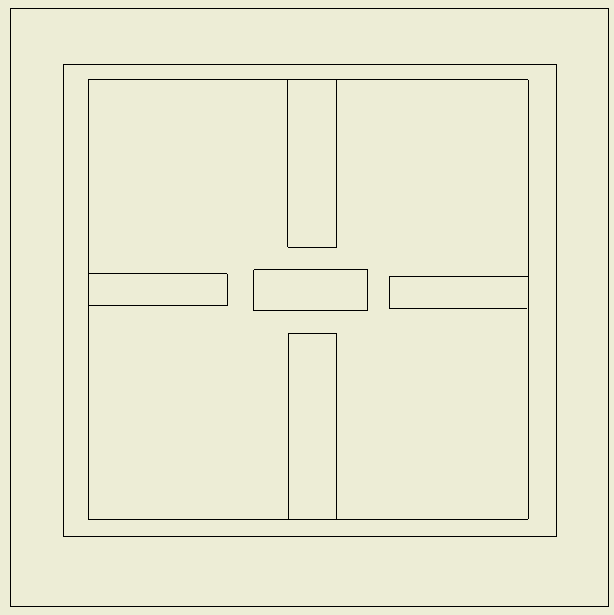
\includegraphics[width=\textwidth]{UnitCell.PNG}};
 \draw(7.65,8) node{$\ell$};
 \draw(0.55,8) node{a};
 \draw(14.65,8) node{a};
 \draw(7.65,0.55) node{a};
 \draw(7.65, 14.65) node{a};
 \draw(9.35,8) node{$g_2$};
 \draw[->, thick, black](7.4,0.55) -- (0.4, 0.55);
 \draw[->, thick, black](8,0.55) -- (14.9, 0.55);
 \draw(5.95,8) node{$g_2$};
 \draw(7.70,8.75) node{$g_1$};
 \draw(7.70,7.25) node{$g_1$};
\end{tikzpicture}
\end{figure}
\noindent
Within this unit cell, at the center, with that being defined as $\ell$ for measuring the width of the charge center, and $g_1$ for measuring the distance of the vertical most piece of the unit cell to the charge center in this case. the parameter $g_2$ in this case for measuring the distance of the horizontal most pieces of the Metamaterial unit cell and there distance from the charge center, which in this case is $\ell$. We then have the parameter, $a$, which is the width and height of the unit cell, which in this case is $a$, which shows the outside width and height of the unit cell shown in the picture above mainly. When this unit cell was being designed, several reasons were taken in to account, which resulted in the design above. The first one of these reasons is mainly due to the fact that for the unit cell to be efficient at reflecting the Quasistatic Magnetic Field, the charge center of the unit cell, in this case $\ell$, had to be 
\subsection*{COMSOL Simulations}
For the simulations for this project within COMSOL, that being the version of COMSOL being 5.2A as the version of COMSOL used for the simulation part of this project. The first simulation done was simulating the Quasi-static magnetic field generator, and the field itself when generated. For this simulation, the main generator, here will be defined as $\phi_c$, with the purpose of the c subscript defining the center generator and Quasi-static magnetic field center point. Then a cylinder was created with the length parameters for the height of the generator being defined as $\Delta$l $\approx$ 2.4384 m, and the radius of the generator being defined as $\Delta$r = 0.75 m. The Cylinder was then split along the center to define two separate domains to add simulation parameters to certain boundaries of the cylinder, and other parts of the Cylinder as well. Next, boundaries of the cylinder were defined for the Quasi-static magnetic field generator, and other components, were defined to have certain parameters for the COMSOL Simulation of the Quasi-static Magnetic Field within COMSOL. These boundaries were mainly meant to define some of the simulation parameters that were used later on used in COMSOL. Then for the Quasi-Static Magnetic Field Simulations within COMSOL, what was next defined was parameters for the domains of the cylinder, this being the Quasistatic Magnetic field generator that was simulated in COMSOL, had domain parameters defined for it, which are different from boundaries parameters due to them defining a large section of the cylinder used for the Quasistatic Magnetic field generator and that simulation when it was done. Once the simulation for that had been done, taking the results was done by COMSOL, and exporting the visual graphs that were created by COMSOL, and the data as a .txt file. This was also done for the other simulations that were done within COMSOL, such as the Metamaterial unit cell, and the simulation of the Quasistatic Magnetic Field around the unit cell. This was mainly done by taking the design I had from Autodesk Inventor for the Metamaterial unit cell, and re-sketching that in COMSOL, and once this was done, all of the separate parts sketched were reunited as one single piece in COMSOL. Once this was done, all of the necessary boundary parameters for the Material were added, along with an Artificial Material created in COMSOL using the Material manager to do so. Once this was done, simulations were ran with the results for the Electric Field Normal, $S11$ and $S21$ parameters were obtained as well, along with the impedance of the $S11$ and $S21$ parameters being obtained as well, which were all graphed onto a smith plot once the simulations were complete and finished within COMSOL Multiphysics itself, with the graphs being exported as a .txt file, and the graphs obtained from the COMSOL simulations as .png files. This was mainly all that was done for the simulations of this project, that were done for the simulation portion of this project within COMSOL Multiphysics 5.2a as the software used to conduct simulations in this project.
\section*{Results}
Below is all the data collected for this project from the simulations within COSMOL that were successful, those being the electric field normal, and along with the S-Parameter graphs as well, which came from the Successful simulate that the electric field normal did. Along with that, what else is shown is mainly the one dimensional form of the electric field normal graphed on a one dimensional line graph in this case.
\begin{figure}[H]
	\centering
	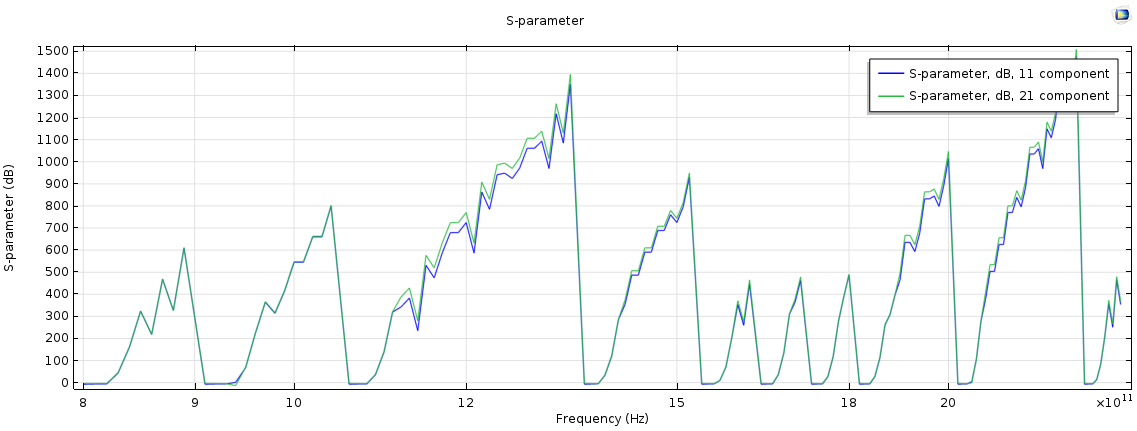
\includegraphics[width=\textwidth]{SParameterGraph1D.png}
	\caption{The Figure above shows the graph for the 2 S-Parameters used within the simulation, with those being the S11 Parameters and S21 Parameters}
	\label{test111}
\end{figure}
\noindent
The figure above mainly displays the results of the COMSOL Simulation for the S-Parameter. The S-Parameter can be seen to have 2 Parameters itself within the graph, this being the $S11$ parameter and $S21$ parameter from the COMSOL simulations on the Metamaterial unit cell. These are of course graphed within the graph above, that being for the $S11$ and $S21$ parameter from the COMSOL simulations that I did on the Metamaterial Unit Cell mainly.
\begin{figure}[H]
	\centering
	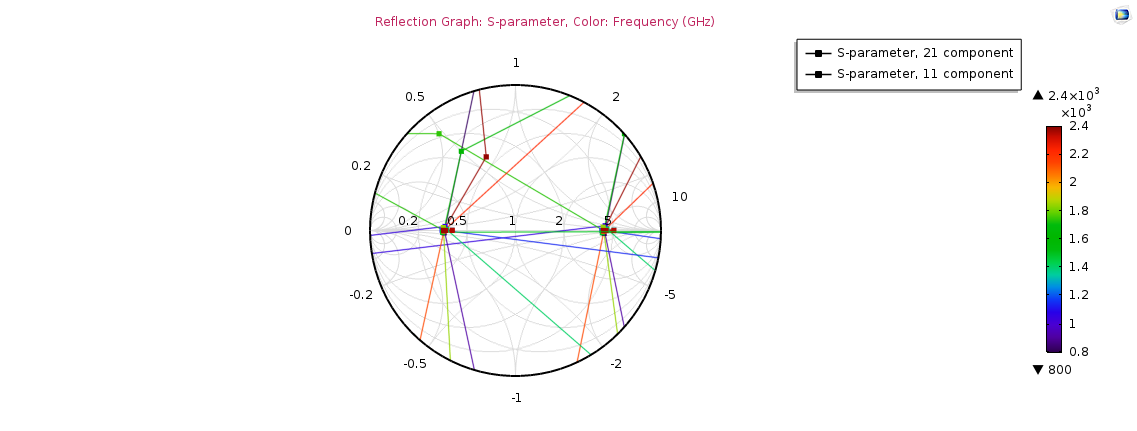
\includegraphics[width=\textwidth]{SmithPlotforReflection.png}
	\caption{This is the Smith Plot for the S21 and S11 Parameter from the simulations within COMSOL.}
	\label{test1112}
\end{figure}
\noindent
What the figure above shows is the Smith Plot Graph for the $S11$ Parameter and the $S21$ Parameter as well for the reflection of the Quasistatic magnetic field off the Metamaterial unit itself, via the impedance of the unit cell of the one used for simulations within COMSOL Multiphysics. This is what the purpose of the graph above mainly does, with it showing this graphed onto a smith plot.
\begin{figure}[H]
	\centering
	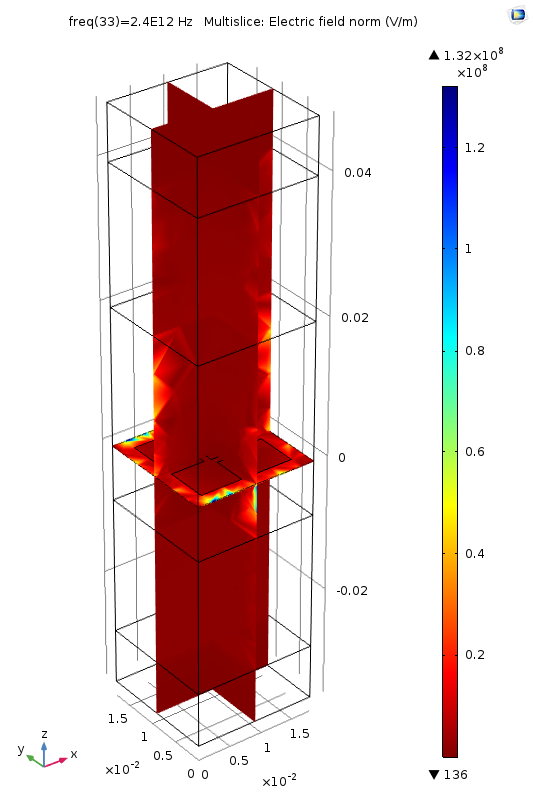
\includegraphics[width=10cm, height=10cm]{ElectricFieldNormalGraphImage2.png}
	\caption{The Figure above is for showing the Electric field normal of the unit cell.}
	\label{test11122}
\end{figure}
\noindent
Within the graph above we have the results of one of the main COMSOL Simulations, with that being for the electric field normal found from simulations done within COMSOL, with the electric field normal being graphed here on the unit cell, but this time with more top like perspective so that the unit cell itself can be seen from the COMSOL Simulations in this case.
\begin{figure}[H]
	\centering
	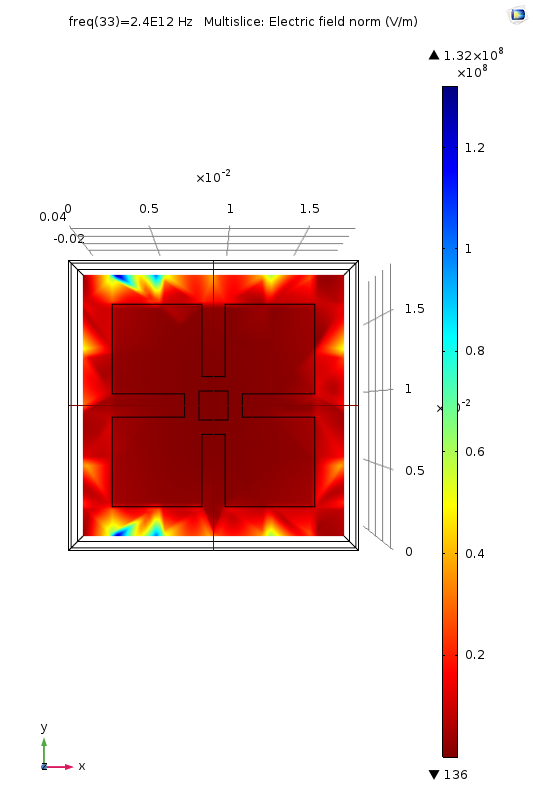
\includegraphics[width=10cm, height=10 cm]{ElectricFieldNormalGraphImage.png}
	\caption{The Figure is above is for the graph of the Electric Field Normal of the Metamaterial unit cell.}
	\label{test2121}
\end{figure}
\noindent
Above is the graph for the electric field normal is shown for the Metamaterial unit cell, with it this time being shown from a top perspective. This was mainly done for showing the unit cell of the Metamaterial, and the electric field normal of it from this top perspective mainly. 
\begin{figure}[H]
	\centering
	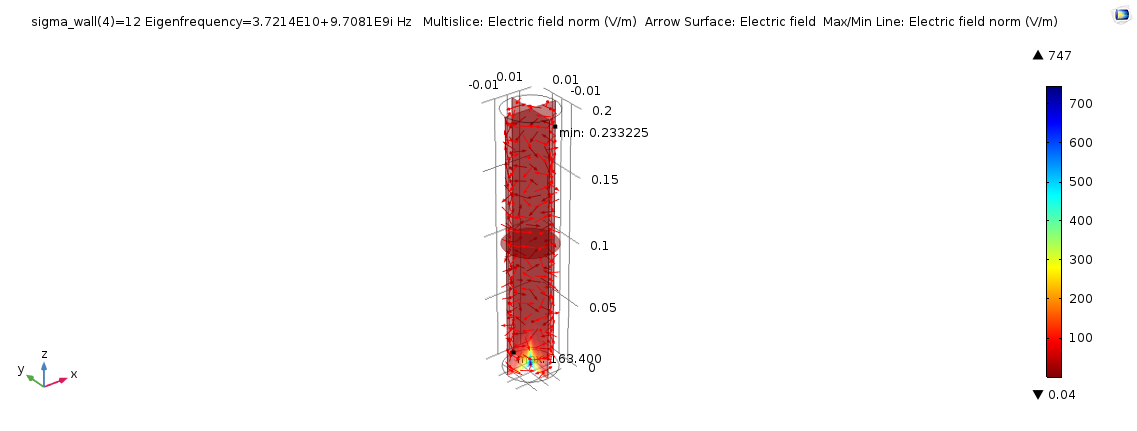
\includegraphics[width=\textwidth]{QuasistaticMagneticFieldVectorDirectionGraphImages.png}
	\caption{The Figure above shows the vector direction of the Quasistatic Magnetic field within the Quasistatic magnetic field .}
	\label{test982}
\end{figure}
\noindent
The Graph above that was just shown is the simulation of the Quasistatic magnetic field, mainly showing the vector direction of the Quasistatic magnetic field that is inside the Quasistatic magnetic field generator. This is mainly shown by the arrows shown in the graph, which are mainly showing the vector direction of the Quasistatic magnetic field generator. 
\begin{figure}[H]
	\centering
	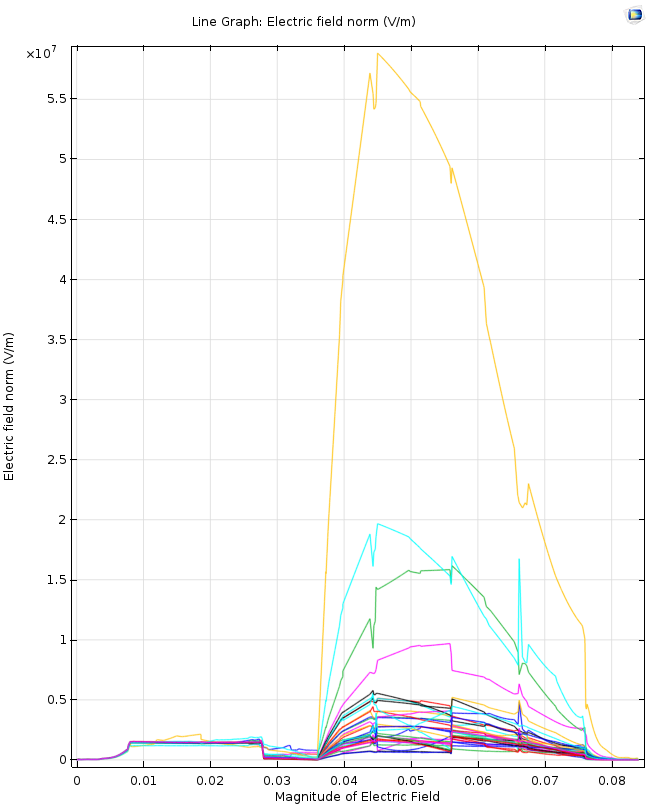
\includegraphics[width=10.5 cm, height=10.5 cm]{OneDElectricFieldNormalGraphImage.png}
	\caption{The Electric field Normal of the Metamaterial Unit Cell graphed in one dimensional form.}
	\label{test8128382}
\end{figure}
\noindent
What the graph above shows is the electric field normal of the Quasistatic Magnetic Field on the unit cell used within COMSOL Simulation. The Data graphed here is mainly the magnitude of the electric field normal at different points on the unit cell itself. The graph above shows this with the units of the Electric field normal, that being the unit of $V/m$ for the Y axis. On the X axis of this graph, we have the magnitude of the electric field normal. Mainly, what is graphed above is the electric field normal in a one dimensional line graph form in this case. 
\section*{Discussion}
With some of the findings of the Data I had within my project, none stood out that much, but one that stood out in particular were the results I found with my S-Parameter, that being with figure 1 in the results section of this paper. The Reason that I say this is because with the S-Parameter, this being the Scattering Parameter, from the simulations in COMSOL, for $S11$ and $S21$ all appear to be the same, which I was expecting to be much different, with much more of a voltage loss for $S21$, which there wasn't which surprised me mainly due to that. This also can be said with the S-Parameters being involved once again, with this being the Smith Plot this time. The Main reason that I say this is that like the S-Parameter Graph, the Same can be said for the Smith Plot, with the two parameters being almost the same in data-points, but rather, with the values for the $S11$ Parameter and $S21$ Parameter. With these results that stand out the most, the possible reason that the $S11$ and $S21$ graphs and smith plot may have looked like this may have been a possible error by me when inputting the simulation parameters into COMSOL, in which a parameter I may have put in for the solver to use caused this to happen as a result, which is possible, but not likely, due to the many times I had to go back and fix the simulation to allow for the simulation to run in the first place, ruling this out as a likely scenario. With models that I have read and seen online, most have had a wide difference in how the two scattering parameters were graphed, that being not close as they were within my case, which saw the two values be nearly identical in where they were on the graph. This probably may have changed if I did more than one simulation on the Unit cell that I designed, that being with different material parameters. In relation to the graph of the Quasi-static Magnetic field Vector Direction Graph, the results of that turned out a mess, mainly due to the error of me inputting the parameters wrong into COMSOL for the simulation, or missing something when adding global parameter and missed the wrong variable in this case, causing for the results of that graph, which in this case is figure number 5 within the results section. Overall, the results that looked the most reasonable in this case would be the Multi-slice graphs that showed the electric field normal and how that interacted with the meta-material unit cell itself, which seemed to have the most reasonable outcome in terms of data.
\section*{Conclusion}
In conclusion, for my project, the results I obtained, the mathematical modeling done, and the COMSOL simulations that were done for this project.Simulations were done in COMSOL Multi-physics 5.2a, to obtain results such as the modeled Quasi-static magnetic field vector direction, and other graphs as well, such as the S-Parameter as well, with the rate of reflection and what was reflected off the meta-material unit cell designed for the receiver, and whether that would be an efficient method of allowing truly mobile wireless charging on a large scale, rather than what it is today, which can be found to be an extremely inconvenient method of wireless charging your device. The data that I received from these simulations however to show that this may not be the case yet, possibly due to the design of the Meta-material unit cell, with how it was designed, which showed this process of making wireless charging to be more efficient with the use of Meta-materials and Quasi-static magnetic fields in this, due to the data that I received from my COMSOL simulations, disproving my hypothesis for my project in the end.
\section*{Acknowledgments}
Relating to any Acknowledgments that I have for anyone for making my project possible and for it succeeding mainly, I would like to thank my scientific research teacher, Mrs.Lounsbury, for helping me narrow down my project idea. In this sense, she basically helped me narrow it down from what the project was originally, which was highly impractical, to practical via simulations within COMSOL, and along with this me doing Mathematical modeling of it as well. 
\section*{Appendix}
All of the Python code used for any statistical tests, t-tests, p-values, etc.
\begin{lstlisting}
import pandas as pd
import matplotlib as plt
from scipy.stats import stats

electricfieldnormaldata = pd.read_csv("Electric Normal Graph Data.csv")
electricfieldnormaldata.describe()
\end{lstlisting}
\begin{lstlisting}
import pandas as pd
import matplotlib as plt
from scipy.stats import stats

dataset = pd.read_csv("VectorArrowDirection - Quasistatic Magnetic Field Vector Arrows Data for Graph.csv")
dataset.describe()
\end{lstlisting}
\begin{lstlisting}
import pandas as pd
import matplotlib as plt
from scipy.stats import stats

dataset = pd.read_csv("MultiSliceDataFromQSField - Quasistatic Magnetic Field Vector Direction Graph Multislice Data.csv")
dataset.describe()
\end{lstlisting}
\begin{lstlisting}
import pandas as pd
import matplotlib as plt
from scipy.stats import stats

dataset = pd.read_csv("Reflection on Metamaterial Graph 1D Data - Reflection on Metamaterial Graph 1D Data.csv")
dataset.describe()
\end{lstlisting}
\begin{lstlisting}
import pandas as pd
import matplotlib as plt
from scipy.stats import stats

dataset = pd.read_csv("Reflection on Metamaterial Graph 1D Data - Reflection on Metamaterial Graph 1D Data.csv")
dataset.describe()
\end{lstlisting}
\begin{lstlisting}
import pandas as pd
import matplotlib as plt
from scipy.stats import stats

dataset = pd.read_csv("SParameter Data - S Parameter Graph 1D Data.csv")
dataset.describe()
\end{lstlisting}
\begin{thebibliography}{999}
	\raggedright
	\bibitem{quasistatic}
	Chabalko, M. J., Shahmohammadi, M, Sample, A. P.
	(2017, 02),
	\emph{Quasistatic Cavity Resonance for Ubiquitous Wireless Power Transfer}.
	Plos One, 12(2), 
	\url{doi:10.1371/journal.pone.0169045}
	
	\raggedright
	\bibitem{elecimedance}
	Electrical impedance
	(2018, November 12),
	Retrieved from,
    \url{https://en.wikipedia.org/wiki/Electricalimpedance}
    
    \raggedright
    \bibitem{wirelssschagringexplained}
    Mearian, L.
    (2018, March 28).
    \emph{Wireless charging explained: What is it and how does it work?}
    Retrieved from,
    \url{https://www.computerworld.com/article/3235176/mobile-wireless/wireless-charging-explained-what-is-it-and-how-does-it-work.html}
    
    \raggedright
    \bibitem{metamats}
    Institute of Physics.
    (n.d.).
    \emph{Metamaterials},
    Retrieved from,
    \url{http://www.iop.org/resources/topic/archive/metamaterials/}
	
\end{thebibliography}
\end{document}